\documentclass[12pt]{article}

% Science template formatting (see science_template.tex)
\usepackage{newtxtext,newtxmath}
\usepackage{graphicx}
\usepackage[letterpaper,margin=1in]{geometry}
% Double line spacing, including in captions
\linespread{1.5} % For some reason double spacing is 1.5, not 2.0!
\frenchspacing

% Abstract: quotation style, no heading
\renewenvironment{abstract}
	{\quotation}
	{\endquotation}

\date{}
\renewcommand\refname{References and Notes}

% Figure and Table labels in bold
\makeatletter
\renewcommand{\fnum@figure}{\textbf{Figure \thefigure}}
\renewcommand{\fnum@table}{\textbf{Table \thetable}}
\makeatother

\usepackage{scicite}
\usepackage{url}

% Additional packages needed for this manuscript
% Note: Template uses \cite (from scicite). \citep replaced with \cite for compatibility.
\usepackage{amsmath}
\usepackage{amsfonts}
\usepackage{bm}
\usepackage{booktabs}
\usepackage{caption}
\usepackage{hyperref}
\usepackage{lineno}
\setlength{\emergencystretch}{1em}
\usepackage[title]{appendix}
\newenvironment{oldappendices}{\begin{appendices}}{\end{appendices}}
% Math shorthand (from macros.sty)
\newcommand{\A}{\mathbf{A}}
\newcommand{\D}{\mathbf{D}}
\newcommand{\R}{\mathbb{R}}
\newcommand{\Z}{\mathbf{Z}}
\newcommand{\f}{\mathbf{f}}
\newcommand{\x}{\mathbf{x}}


%%%%
\captionsetup{font=small}

% %% as per the requirement new theorem styles can be included as shown below
% % \theoremstyle{thmstyleone}%
% \theoremstyle{plain}%
% \newtheorem{theorem}{Theorem}%  meant for continuous numbers
% %%\newtheorem{theorem}{Theorem}[section]% meant for sectionwise numbers
% %% optional argument [theorem] produces theorem numbering sequence instead of independent numbers for Proposition
% \newtheorem{proposition}[theorem]{Proposition}% 
% %%\newtheorem{proposition}{Proposition}% to get separate numbers for theorem and proposition etc.

% \theoremstyle{definition}%
% \newtheorem{example}{Example}%
% \newtheorem{remark}{Remark}%

% \theoremstyle{remark}%
% \newtheorem{definition}{Definition}%

% \raggedbottom
% %%\unnumbered% uncomment this for unnumbered level heads

% Store the title in a variable for reuse in the supplement (otherwise \maketitle deletes it)
\def\scititle{Advancing paleobotany with AI-guided expert fossil leaf identification}
\def\scishorttitle{AI cracks the fossil leaf code}

\begin{document}
\title{\bfseries \boldmath \scititle}
\author{
	I.~F.~Rodriguez$^{1\dagger}$,
	T.~Fel$^{1,2\dagger}$,
	G.~Gaonkar$^{1}$,
	M.~Vaishnav$^{1}$,
	H.~Meyer$^{3}$,
	P.~Wilf$^{4}$,
	T.~Serre$^{1\ast}$\and
	\small$^{1}$Department of Cognitive \& Psychological Sciences, Brown University, Providence, RI, USA.\and
	\small$^{2}$Kempner Institute, Harvard University, Boston, MA, USA.\and
	\small$^{3}$Florissant Fossil Beds National Monument (Emeritus), National Park Service, Florissant, CO, USA.\and
	\small$^{4}$Department of Geosciences, Pennsylvania State University, University Park, PA 16802, USA.\and
	\small$^\ast$Corresponding author. E-mail: thomas\_serre@brown.edu\and
	\small$^\dagger$These authors contributed equally to this work.
}

\maketitle
\linenumbers

\noindent\textbf{Short title:} \scishorttitle

\noindent\textbf{One-sentence summary:} A deep learning system that generates synthetic fossils from modern leaves identifies fossil angiosperm families with high accuracy and reveals interpretable diagnostic morphology, unlocking paleobotanical dark data.

\begin{abstract} \bfseries \boldmath
    Fossil angiosperm leaves hold abundant but untapped data about evolutionary history and ancient ecosystems, yet identifying them remains manual, error-prone, and expert-dependent, leaving most collections as paleobotanical ``dark data.'' Scarcity of vetted fossil specimens, absence of fossils for most families, and preservation artifacts have thwarted machine learning approaches. We present a deep learning system that generates fossil-like images from modern leaves while aligning family-diagnostic features across domains. Tested on ``dicot'' families with vetted fossils from the Florissant Fossil Beds (late Eocene, Colorado), the system achieves 93.2\% top-5 accuracy (vs.\ 3.5\% chance), maintaining 77.3\% even when all fossils from a test family are withheld during training. Concept-based explanations reveal diagnostic morphology, including venation, margin, and leaf base characters, to guide expert review. Applied to 1,177 previously unidentified Florissant specimens, the system provides credible family-level hypotheses for 85.6\%, demonstrating practical decision support for fossil identification.
\end{abstract}

\noindent
Isolated leaves dominate the angiosperm fossil record yet remain notoriously difficult to identify accurately, representing paleobotany's largely untapped source of ``dark data''~\cite{Dilcher_1971}. Historical literature is riddled with botanically incorrect identifications due to the inherent complexity of leaf morphology, insufficient vetted reference samples, and considerable variation in preservation and taxonomy within and across fossil sites. Consequently, most well-identified fossil leaves represent only a handful of morphologically distinctive families that are well-represented in the literature, leaving the vast majority of angiosperm diversity in the fossil record unrecognized~\cite{Hickey1975, Wilf2008FossilLeaves}. 

Accurate fossil leaf classification is crucial because leaf fossils provide essential data for interpreting evolutionary radiations and extinctions, biome evolution, plant-animal interactions, biogeography, and biotic responses to climate change~\cite{Giraldo2025, Hickey1977, Johnson1989, Kooyman2014, Wing2005}. At the family level---the traditional first step for most extant and fossil plant identifications---classification provides a stable taxonomic anchor, since nearly all fossil plants represent extinct species, and many belong to extinct genera. Our previous work demonstrated that machine learning can successfully classify modern cleared leaves at the family level~\cite{wilf2016leaves}. However, these approaches fail for fossils because fossilization—through compression, mineralization, and fragmentation—creates an effectively new visual domain.

While machine learning has shown promise for classifying modern leaves~\cite{wilf2016leaves, Barre2017LeafNet,machinelearningspecies,Adaime2024}, no method has successfully bridged the domain gap to fossilized specimens. Recent advances in deep learning---particularly generative models for data augmentation and domain adaptation techniques---offer potential solutions to this challenge. However, realizing their potential requires addressing several interconnected obstacles: learning family-diagnostic morphology at multiple spatial scales, generating synthetic fossils that preserve family-specific features while enabling generalization to families lacking fossil training examples, and aligning modern and fossil representations despite extreme visual differences. We address these challenges through a unified framework that jointly optimizes synthetic fossil generation, cross-domain representation alignment, and family classification in a single end-to-end training process.

To control for taphonomic variability, we focus here on a single, exceptionally well-documented fossil locality, the late Eocene Florissant fossil beds, currently preserved as Florissant Fossil Beds National Monument. Preserved under relatively consistent lacustrine conditions~\cite{Harding2000}, the Florissant flora represents one of the best-understood Cenozoic plant assemblages, documented in MacGinitie's seminal 1953 monograph~\cite{mcginitie1953fossil} and subsequently expanded and revised through decades of systematic research~\cite{manchester1983fagopsis,Manchester2001Florissant,Jia2014Cercis,Herendeen2019Arcoa}. The Meyer et al.~\cite{florissant} digital archive of Florissant fossils, recently recompiled by the National Park Service and the University of Colorado Museum of Natural History as part of a large open-access dataset of fossil leaves, in addition to cleared and X-rayed leaves from other collections, totaling more than 37,000 images~\cite{wilf2021dataset}, provides a uniquely rich and accessible foundation for AI applications in paleobotany. From this resource, we curated 2,923 taxonomically vetted Florissant fossil leaves spanning 16 angiosperm families, each with at least 5 specimen images (an additional 6 families had fewer than 5 specimens and were excluded from model evaluation). An additional 1,177 evaluable Florissant specimens lacking confident family assignments under modern standards were reserved to assess the system's practical utility ~\cite{methods}.

A central obstacle for fossil classification is that most families have few or no vetted fossil training exemplars. To address this, we employ a generative approach~\cite{zhang2023adding} that simultaneously learns to synthesize fossil-like images from modern leaves while training a classifier—both optimized together in a unified end-to-end process. The system is trained on modern leaves spanning 142 families, a limited set of vetted fossils, and synthetic fossils generated during training, with the generator learning to preserve family-specific morphological features while expanding the diversity and taxonomic coverage of training material (Fig.~\ref{fig:SI_Full_system}). This joint optimization achieves high classification accuracy---including robust generalization to families with no fossil training examples---demonstrating that generative AI can overcome fundamental data scarcity in macrofossil paleobotany. Interpretability methods reveal botanically meaningful morphological features driving classifications, and application to previously unidentified Florissant specimens demonstrates practical utility for unlocking paleobotanical dark data.



\subsection*{Classification of fossil leaves}

To quantify classification performance, we evaluated our approach on 2,923 taxonomically vetted Florissant fossil leaves spanning 16 families, alongside 32,913 modern cleared and X-rayed leaves from 142 families. Because vetted fossils are not available for most of the 142 families, we tested performance in two scenarios~\cite{methods}: in-distribution (ID), where fossil training data was available for test families, and out-of-distribution (OOD), where all fossils from test families were withheld during training. 

Baseline models trained only on real specimens achieved modest performance when tested on families seen during training (ID: 67.3\%), but failed when tested on unseen families (OOD: 3.8\%, barely above the 3.5\% chance; Fig.~\ref{fig:system}A), revealing the profound visual differences between modern and fossil specimens. Systematic analysis revealed four major obstacles that, once addressed, dramatically improved performance: (i) spurious shortcuts that prevented focus on diagnostic morphology, (ii) the need to capture family-diagnostic features across multiple spatial scales, (iii) domain misalignment between modern and fossil representations, and (iv) extreme data scarcity for most families. We addressed each obstacle systematically.



Neural networks often exploit spurious correlations—shortcuts—between image backgrounds and class labels. In scientific applications, this leads models to rely on data acquisition artifacts rather than meaningful biological features~\cite{Brown2023ShortcutTesting,Hill2024ShortcutRisk,Shahamatdar2024Deceptive}. To assess our model's robustness against such shortcuts, we computed attribution maps using saliency methods from our custom Xplique toolbox~\cite{fel2022xplique}. Visual inspection revealed that the model sometimes based decisions partly on background elements, annotations, and text on slides rather than leaf morphology. Although these shortcuts might improve in-distribution accuracy, they likely harm out-of-distribution generalization to novel collections with different imaging conditions. To address this, we fine-tuned the Segment Anything Model (SAM)~\cite{kirillov2023segment} using manually annotated, cleared leaf images, enabling effective leaf segmentation from backgrounds. After applying this model to mask backgrounds across the entire dataset (Fig.~\ref{fig:system}B), classification accuracy remained high, with modest but consistent improvements in both ID (70.1\%) and OOD (4.6\%) scenarios. Crucially, attribution maps confirmed that the segmented model predominantly relies on leaf morphology rather than background artifacts (Fig.~\ref{fig:attribution_maps}).


% \enlargethispage{5mm}
Eliminating shortcuts alone was insufficient—the model also needed to capture biologically meaningful features across multiple spatial scales~\cite{Hickey1975}, from macroscopic traits such as overall shape and margin to mesoscopic patterns such as venation. We decomposed each input image into five representations at different resolutions to capture this hierarchical structure (Fig.~\ref{fig:system}C). This multi-scale approach improved classification performance in both ID (75.1\%) and OOD (8.7\%) scenarios.

Despite these improvements, analysis of the model's learned representations revealed a fundamental problem: fossil and modern leaves from the same family were widely separated in the model's embedding space (mean normalized distance = 11.45, SD = 3.1)~\cite{methods}, indicating that the model treated them as distinct domains despite their shared family-level morphology. This separation arose from damage, compression artifacts, and variable preservation in fossils. Uniform Manifold Approximation and Projection (UMAP) visualization revealed this domain gap (Fig.~\ref{fig:system}D, left), illustrating why systems trained only on modern leaves cannot generalize to fossils.

To address this domain shift, we trained the model with an additional constraint that brings fossil and modern leaves from the same family closer in representation space while pushing apart leaves from different families (implemented with a triplet loss)~\cite{methods}. This explicitly shapes the embedding space so that embeddings cluster by family rather than by domain (Fig.~\ref{fig:system}D, right). Residual structure associated with preservation or imaging mode may remain, but it does not impede our main goal---family-level identification---because same-family specimens are still brought into close neighborhoods after alignment. Consistent with this, alignment dramatically reduced cross-domain distances within families (mean normalized distance = 1.72, SD = 0.2) and substantially improved performance in both ID (82.3\%) and OOD (24.6\%) settings, with the largest gains in the OOD scenario where vetted fossil examples were not available during training.

% \enlargethispage{5mm}

The most severe challenge was extreme data imbalance and sparsity: our dataset comprised 32,913 extant and 2,923 fossil leaves---approximately a 10:1 ratio---with no fossil specimens for most families (119 of 142) and insufficient specimens for training in 6 others (with fewer than 5 samples). To address this limitation, we leveraged generative AI by adapting a stable diffusion model based on the ControlNet architecture~\cite{zhang2023adding}. We fine-tuned a ControlNet-based diffusion model to generate realistic fossil images from modern cleared leaves (Fig.~\ref{fig:system}E), training it jointly with our classifier using a combined objective~\cite{methods}. This generative augmentation dramatically improved performance in both ID ($67.3\% \rightarrow 93.2\%$) and OOD ($3.8\% \rightarrow 77.3\%$), substantially narrowing the performance gap. 

Having achieved robust classification across domains, we turned to understanding which morphological features drove the model's predictions—critical for paleobotanical applications. High-performing AI models often function as black boxes, making the rationale behind their predictions difficult to interpret, even though they may encode abundant, novel taxonomic information~\cite{spagnuolo22, wilf2016leaves}. We developed an explainability framework~\cite{fel2024sparks} to decompose the model's internal representations into interpretable visual patterns—discrete morphological features we call ``concepts''—potentially uncovering diagnostic characters that are difficult for human observers to discern~\cite{spagnuolo22}.
Extracting these concepts is challenging because neural networks typically mix multiple visual features within individual processing units. A single neuron might respond to both vein junctions and leaf margins simultaneously, obscuring which feature actually drives classification. To separate these mixed signals, we applied sparse dictionary learning~\cite{holistic}, specifically using a top-k sparse autoencoder~\cite{gao2024scaling,fel2025archetypal}, to decompose the model's internal activations into distinct, interpretable patterns. 

To make these concepts interpretable, we visualized them using two complementary methods: heat maps showing where each concept activates on actual leaf images~\cite{fong2017meaningful,petsiuk2018rise,fel2021sobol}, and synthetic (feature visualization) images revealing the visual patterns that most strongly trigger each concept~\cite{olah2017feature,fel2023unlocking}. Representative examples are shown in Fig.~\ref{fig:concepts}, with additional examples in Figs.~\ref{fig:SI_concepts}--\ref{fig:SI_concepts2}. We then measured how much each concept contributed to classification, assigning each concept an importance score for each family~\cite{holistic}. The complete set of extracted concepts with family-specific importance scores is available online (see Data and Materials Availability). Importantly, these concepts are shared across domains: fossil and extant leaves from the same family activate the same diagnostic features (Fig.~\ref{fig:shared_concepts}).


\enlargethispage{5mm}

To assess real-world utility beyond quantitative benchmarks, we applied the trained system to 1,177 previously unidentified Florissant specimens~\cite{methods}. The model's predictions and accompanying interpretability results were evaluated by the two team paleobotanists (P.W. and H.M.; Fig.~\ref{fig:unknown}). The paleobotanists deemed 543 (46.1\%) classifications as possible matches and an additional 465 (39.5\%) as good candidates, yielding 1,008 credible family-level hypotheses (85.6\% of specimens) warranting further paleobotanical investigation. An extensive list of specimens and model annotations is available (see Data and Materials Availability). Beyond these validation specimens, we developed an interactive web application (see Data and Materials Availability) that enables researchers to upload their own fossil leaf images and obtain family-level predictions with concept-based visual explanations.

\subsection*{Discussion}


We present a robust framework that addresses a central challenge in paleobotany---accurate identification of fossil angiosperm leaves. By synthesizing realistic fossil images from extant leaf data using generative AI, our system achieves high identification accuracy, even for families lacking fossil training examples. Interpretability methods reveal botanically meaningful features that define families across fossil and extant specimens. For extant leaves, this represents the first systematic interpretability analysis of a high-performing angiosperm identification system, surfacing morphological patterns that warrant further botanical investigation. For fossil applications where model failures are inevitable, interpretability enables paleobotanists to assess what features drive individual predictions, supporting informed decisions about when to trust model outputs and when additional scrutiny is needed. Because the current system was trained and evaluated on a single locality with relatively uniform taphonomic conditions, testing across additional fossil deposits with different preservation modes remains an important next step.

Applied to previously unidentified Florissant specimen images, the model generates credible family-level hypotheses for 85.6\% of cases, with the potential to substantially reduce longstanding taxonomic uncertainties in this flora. The extracted visual concepts---capturing venation architecture, margin characters, and leaf base morphology---provide a new vocabulary for characterizing family-diagnostic features across modern and fossil specimens, complementing traditional morphological descriptions. The cross-domain training strategy is generalizable to other well-sampled fossil deposits with diverse taphonomic conditions, positioning this approach for broad application across paleobotany. More broadly, improved taxonomic resolution of fossil floras advances our understanding of plant evolution and the ecological dynamics of ancient terrestrial ecosystems.


%%%%%%%%%%%%%%%% MAIN TEXT FIGURES %%%%%%%%%%%%%%%

% Figure 1: Full-page system overview (image on one page, caption on next)
\begin{figure}[p]
    \centering
    \includegraphics[width=\textwidth,height=0.99\textheight,keepaspectratio]{Figures/Figure1_v13_compat.pdf}
\end{figure}

\captionof{figure}{\textbf{Progressive improvements in fossil leaf classification through four technical innovations.}
\textbf{Top:} Classification accuracy improves from near-chance levels (3.5\%,
black dashed line) as each innovation is added. The final system achieves 91.8\% overall accuracy
(red dashed line; combined performance on modern cleared leaves and fossils), with fossil-specific
performance of 93.2\% in-distribution (ID) and 77.3\% out-of-distribution (OOD). Two evaluation
scenarios test generalization: ID, where the model has seen real fossil examples from test
families during training, and OOD, where test families are represented only by synthetic
fossils during training, challenging the model to classify families it has never seen as real fossils.
\textbf{Panels A--E} illustrate each innovation:
(\textbf{A}) Baseline model using raw leaf images without preprocessing.
(\textbf{B}) Segmentation removes background artifacts (rulers, text, annotations) to isolate
leaf morphology.
(\textbf{C}) Multi-scale analysis processes each leaf at five resolutions, capturing both
overall shape and fine venation details.
(\textbf{D}) Domain alignment via triplet loss brings fossil and modern leaves from the same
family together in embedding space. \textbf{Left:} without alignment, embeddings cluster by
domain (fossil vs.\ modern). \textbf{Right:} with triplet loss, embeddings cluster by family
regardless of domain. Residual structure associated with preservation/imaging mode may persist after alignment, which does not limit family-level classification in our setting but motivates future tests across additional sites and taphonomic conditions.
(\textbf{E}) Synthetic fossil generation provides training data for families lacking real
fossils. \textbf{Top row:} synthetic fossils generated from modern leaves (\textbf{bottom row})
to provide training examples when real fossils (\textbf{middle row}) are unavailable or scarce.}
\label{fig:system}

% Figure 2: Visual concepts
\begin{figure}
    \centering
    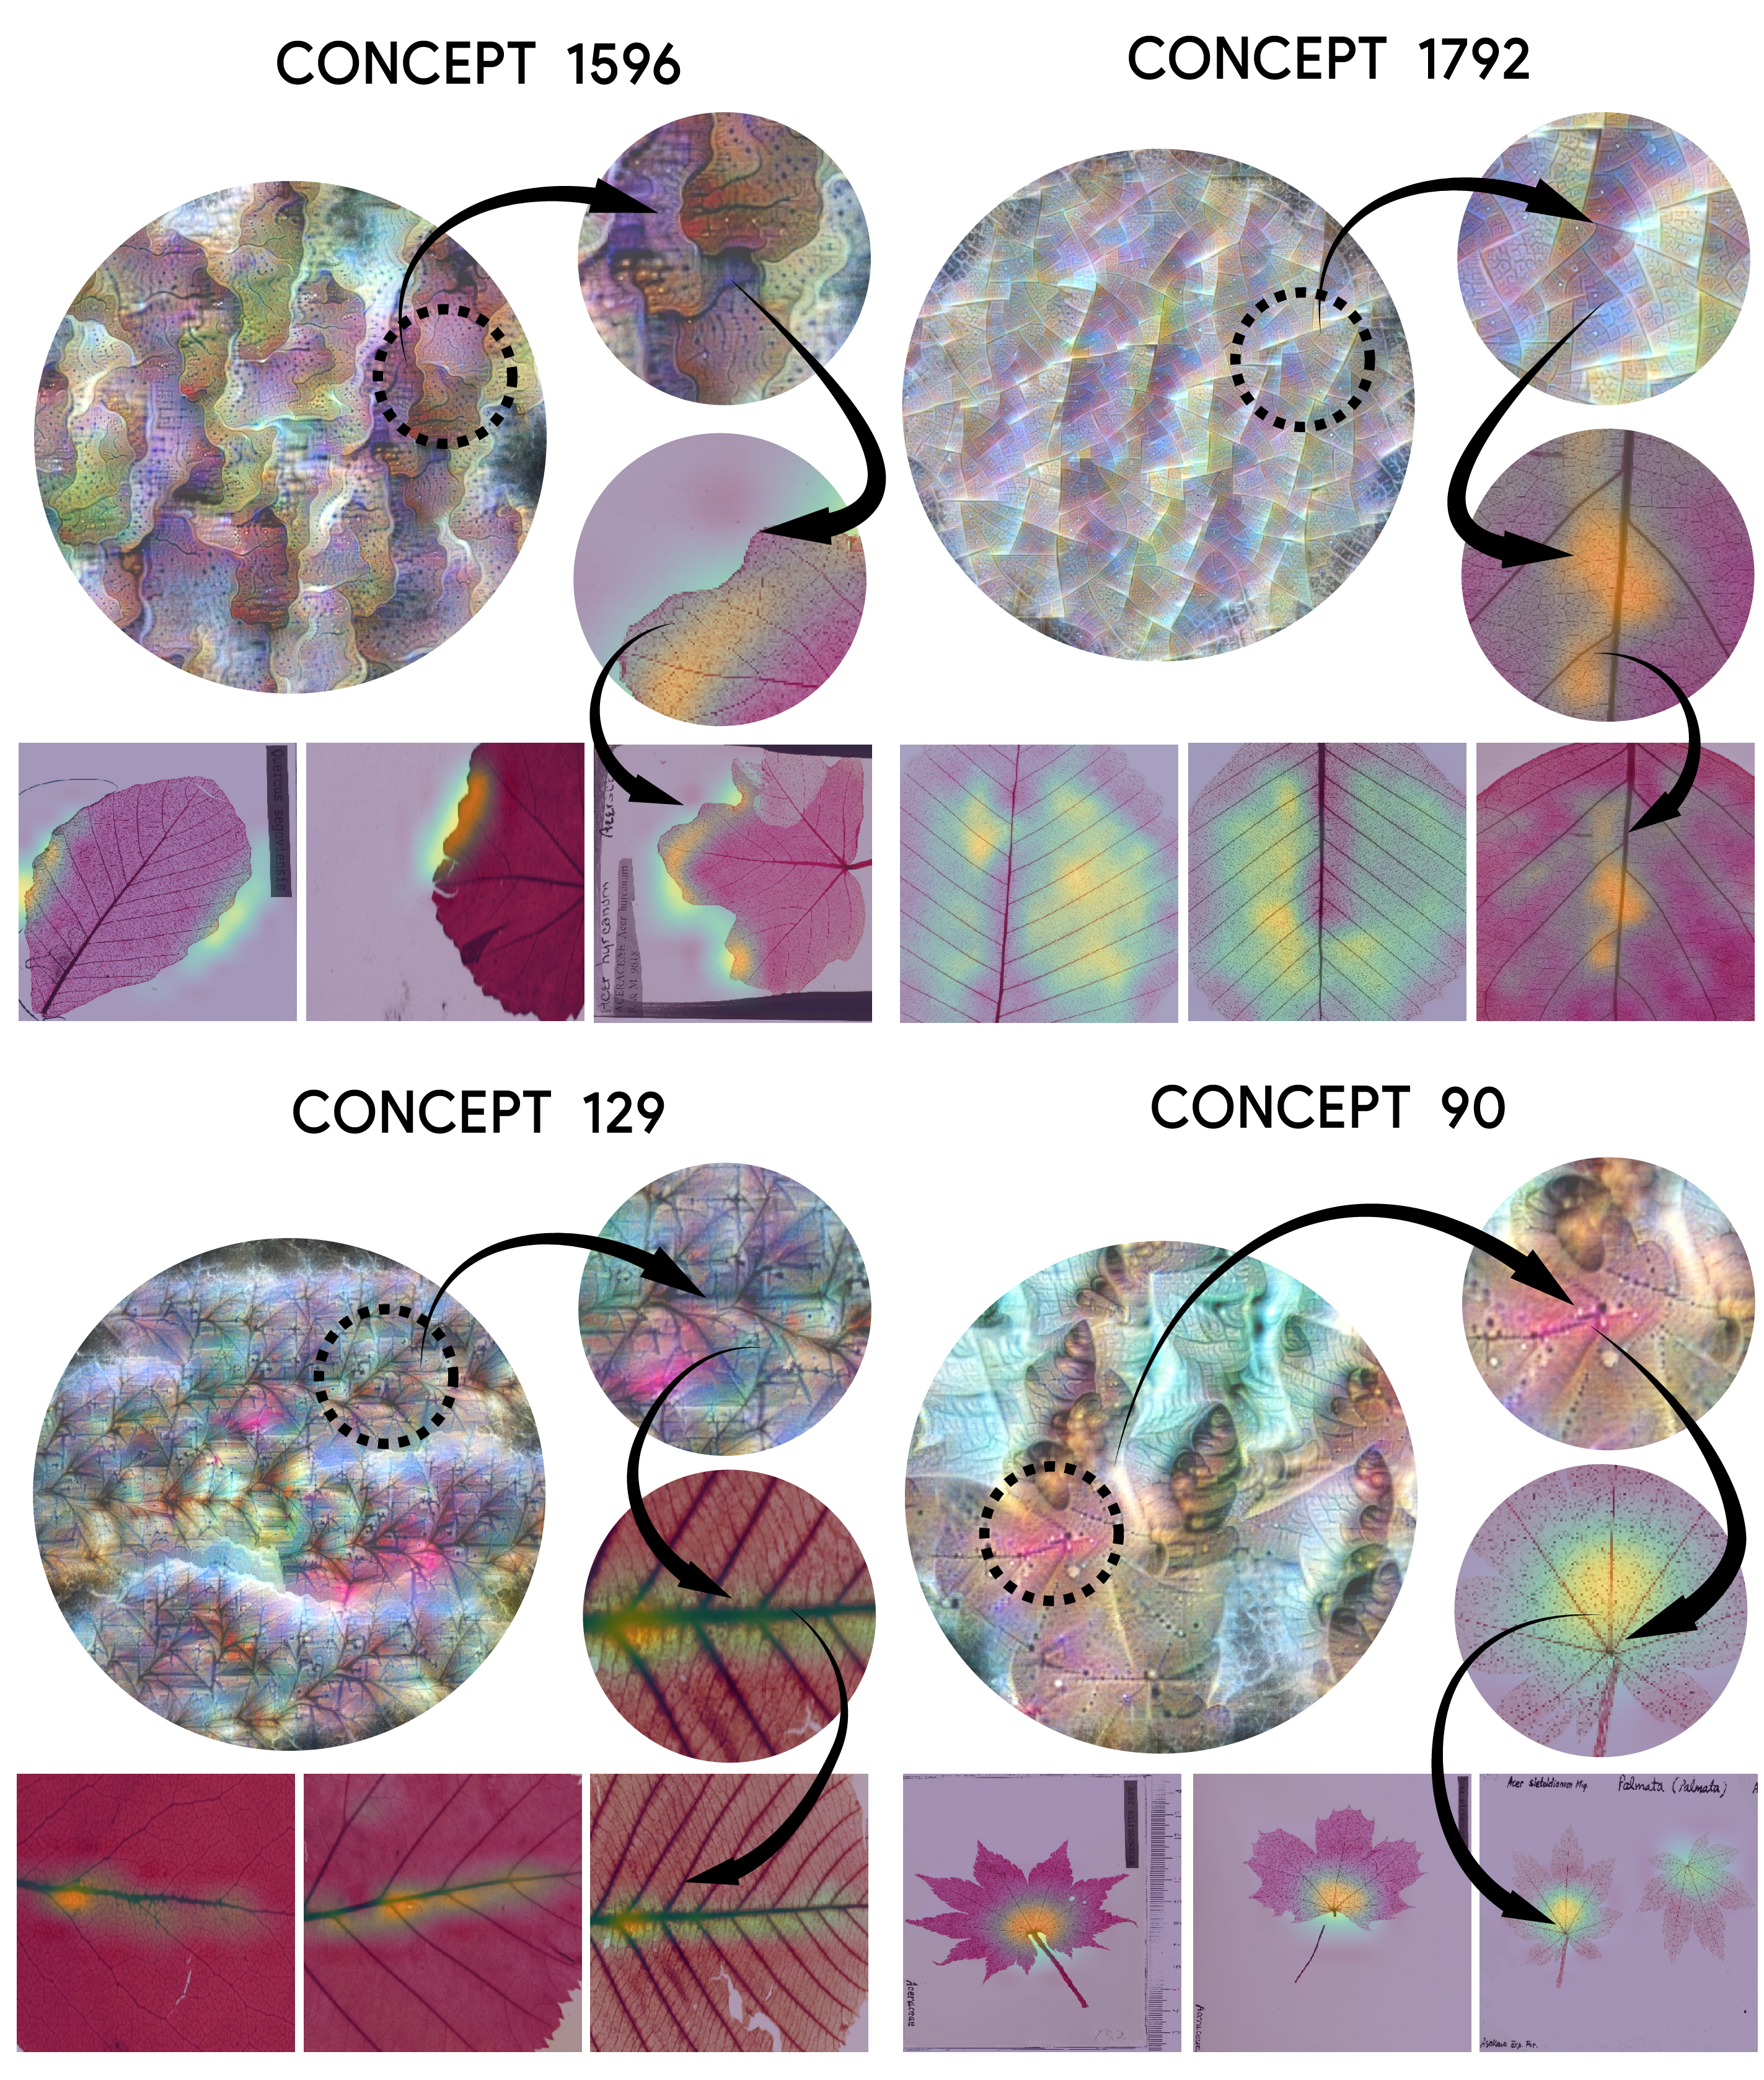
\includegraphics[width=0.7\textwidth]{Figures/Figure_6_v2.jpg}
    \caption{\textbf{Representative visual concepts extracted via sparse dictionary learning.} Four
morphologically distinct concepts are shown: \textbf{Concept 1596} (leaf margins),
\textbf{Concept 1792} (intercostal areas between veins), \textbf{Concept 129} (junctions
between primary and secondary veins), and \textbf{Concept 90} (leaf base). For each concept:
\textbf{leftmost panel} shows feature visualization (synthetic image revealing the minimal
morphological pattern that maximally activates the concept), followed by three attribution
maps (heat maps showing where the concept activates on actual specimens). These concepts are
shared across domains, contributing to the classification of both modern and fossil leaves
(Fig.~\ref{fig:shared_concepts}).}
    \label{fig:concepts}
\end{figure}

% Figure 3: Domain-invariant concepts
\begin{figure}
    \centering
    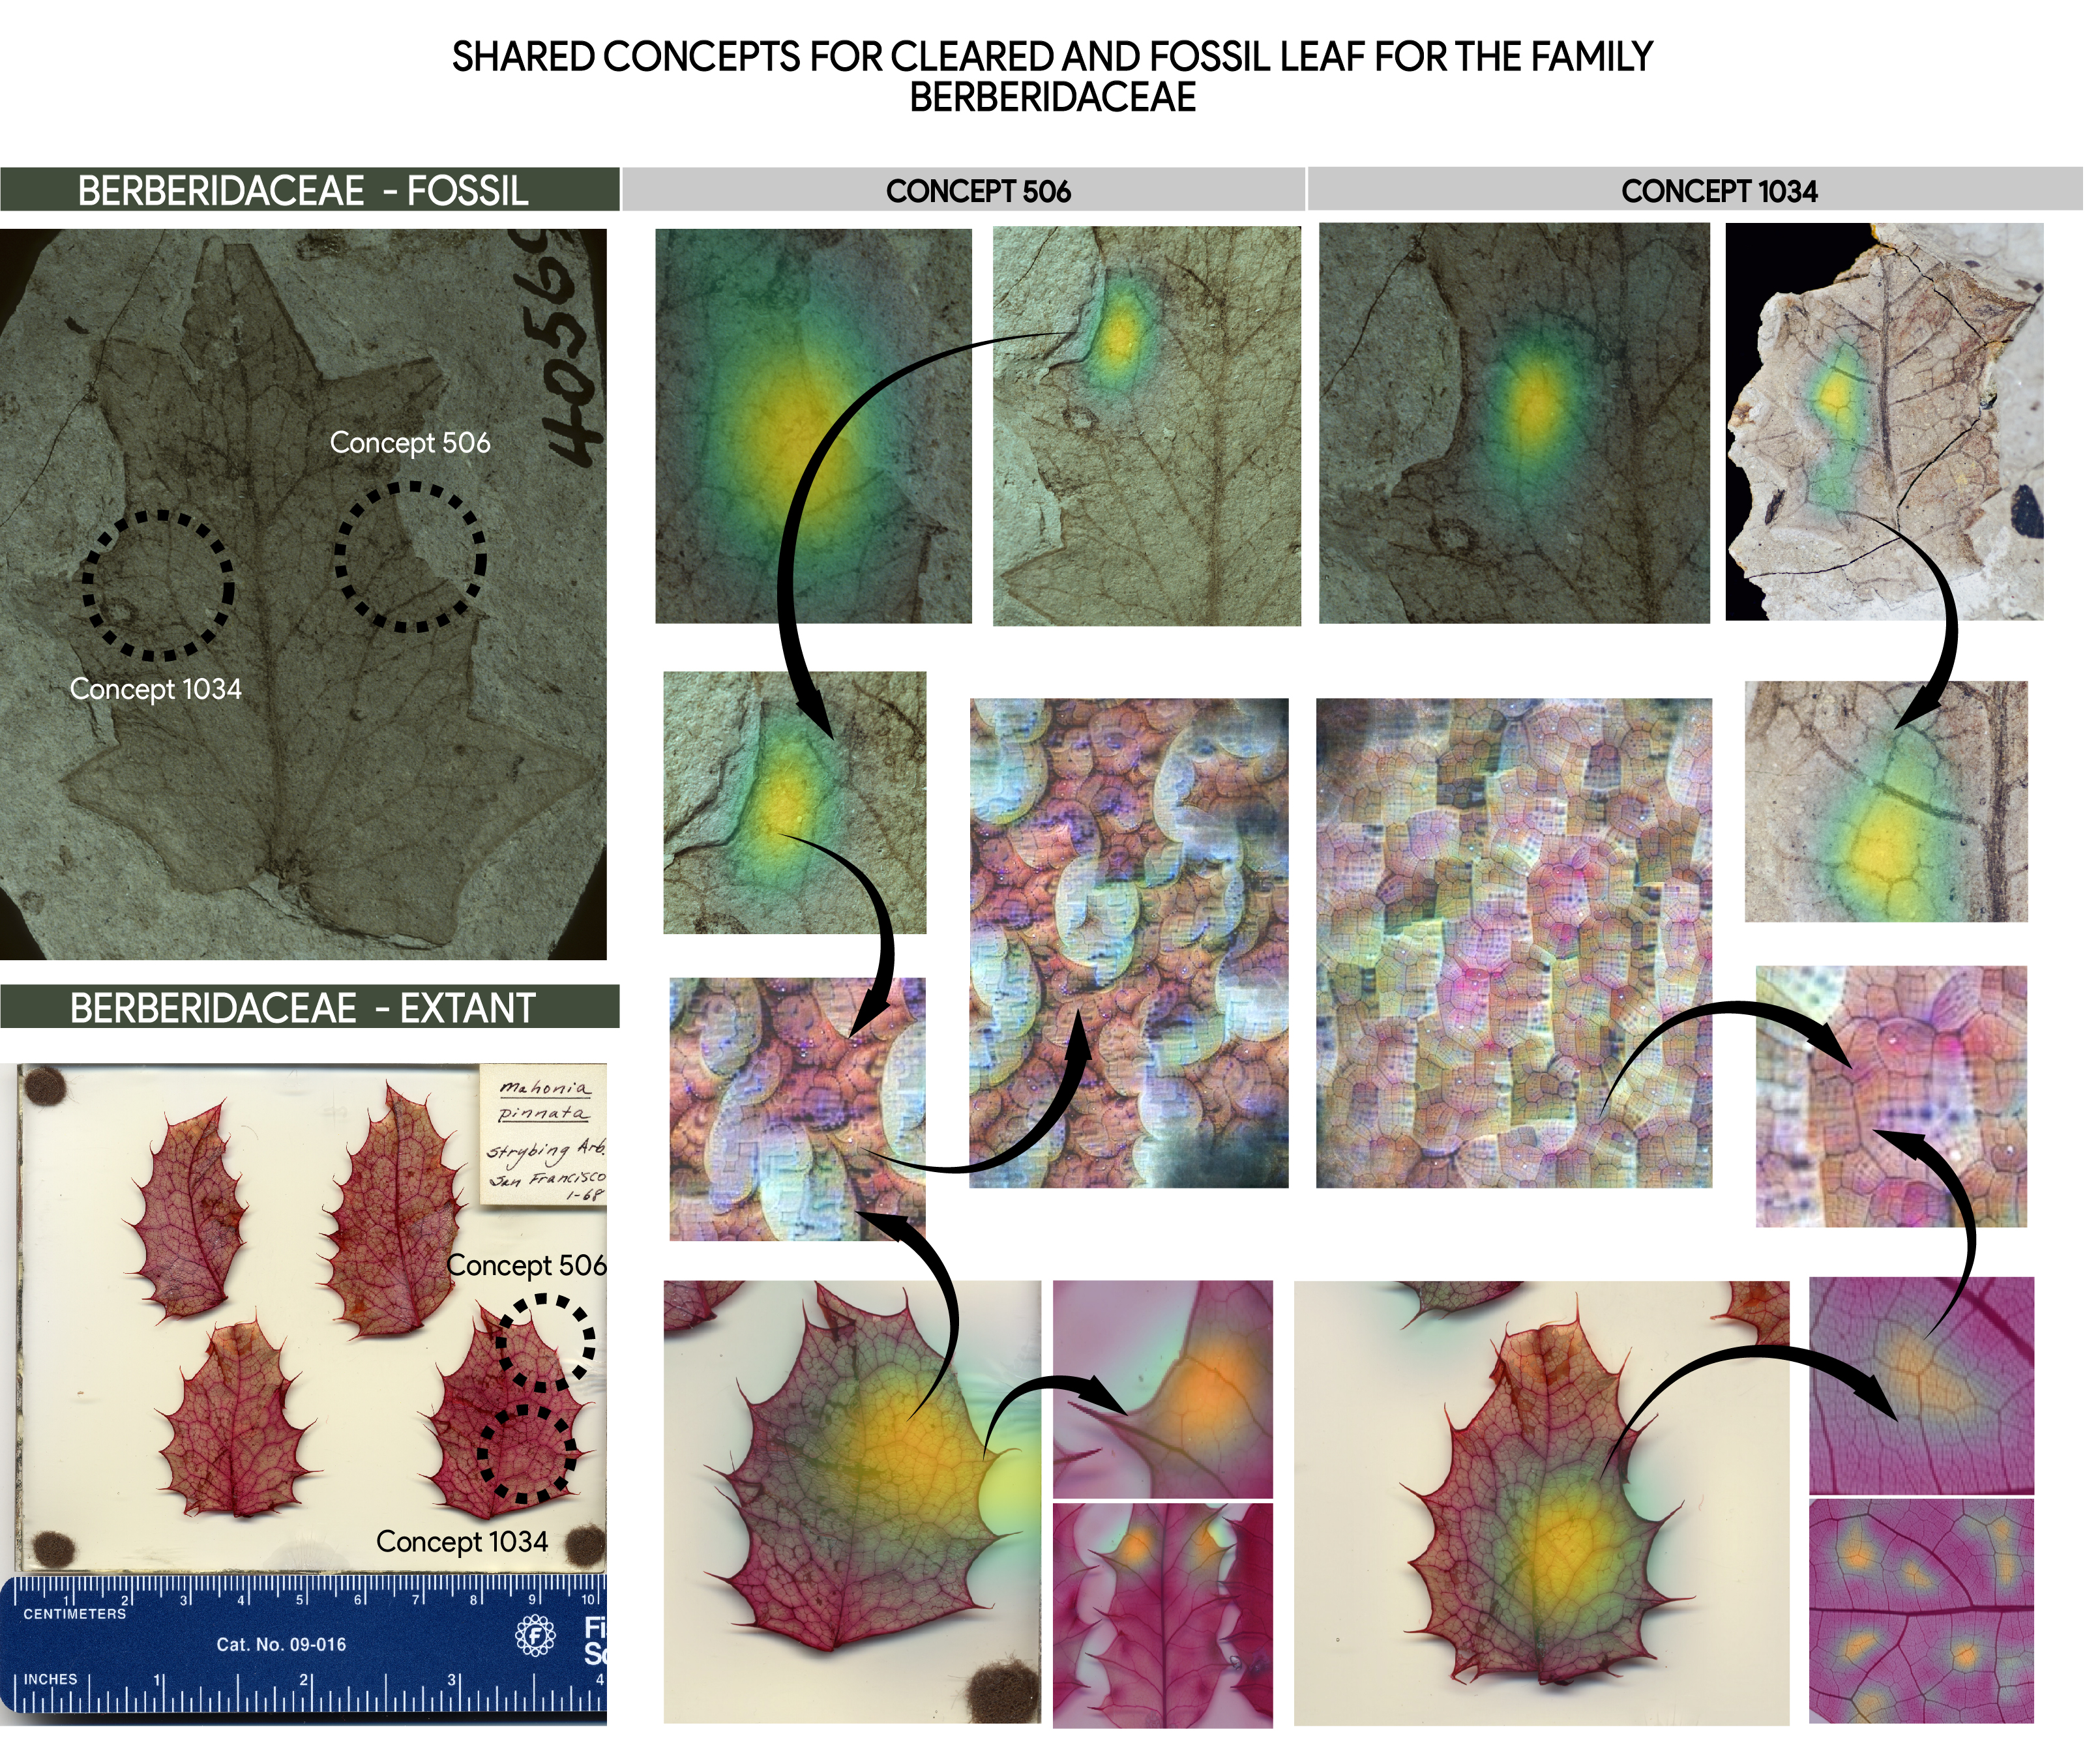
\includegraphics[width=\textwidth]{Figures/Figure_3_v3.jpg}
    \caption{\textbf{Domain-invariant concepts drive classification across modern and fossil specimens.}
    Examples from the family Berberidaceae demonstrate that the same visual concepts activate on
    both compression fossils (\textbf{top row}) and cleared modern leaves (\textbf{bottom row}).
    Each column shows a different concept with its feature visualization (\textbf{leftmost in each
    group}) and attribution maps on modern and fossil specimens. The triplet-loss training
    explicitly aligns these shared morphological features across domains, enabling the model to
    classify fossils from families lacking fossil training examples. Concept numbers and
    morphological features are identified above each column.}
    \label{fig:shared_concepts}
\end{figure}

% Figure 4: Unknown specimen predictions
\begin{figure}\vspace{-5mm}
    \centering
    \includegraphics[width=0.65\textwidth]{Figures/Figure_2_V11.pdf}
    \caption{\textbf{Model predictions for three previously unidentified Florissant fossil specimens.}
For each specimen (\textbf{left}), the model provides: (\textbf{middle}) top-5 family
predictions ranked by confidence, and (\textbf{right}) the most diagnostic visual concepts
driving the classification with attribution heat maps showing spatial localization.
Morphological features include secondary-vein arrangement, marginal dentation (tooth shape
and distribution), reticulate areolation patterns, and primary-secondary vein junctions.
These concept-based explanations enable paleobotanists to evaluate prediction credibility
and guide taxonomic assessment.}
    \label{fig:unknown}
\end{figure}


\clearpage

% \bibliography{sn-bibliography,xai,dictionary_learning}
\bibliography{all_references_corrected}
\bibliographystyle{sciencemag}



\section*{Acknowledgments}
Yuxian Wang contributed to the development of the interactive web application for fossil leaf classification. Sarah Allen provided image samples. Paula Vargas assisted with final figure editing, and Jacob Rose with the initial curation of the image datasets. We thank Edward Spagnuolo, Teng-Xiang Wang, L. Alejandro Giraldo, and Steven Manchester for helpful discussions on the paleobotanical aspects of this work, and Drew Linsley for comments on the manuscript.

\paragraph*{Funding:}
This work was funded by an NSF FRES grant (EAR-1925481 to T.S. and EAR-1925755 to P.W.). Computing support was provided by the Center for Computation and Visualization (CCV) (via NIH Office of the Director grant S10OD025181). We also acknowledge the Cloud TPU hardware resources that Google graciously provides through the TensorFlow Research Cloud (TFRC) program.

\paragraph*{Author contributions:}
P.W. and T.S. conceptualized and supervised the research. I.F.R., M.V., and T.F. developed the deep learning architecture and training system. T.F. and T.S. developed the interpretability and explainability framework. G.G. conducted quantitative analyses, developed the interactive web application and visualization tools, and created online resources. P.W. and H.M. curated and taxonomically vetted the fossil dataset and provided expert assessments of AI-based identifications for unidentified specimens. I.F.R., T.F., P.W., and T.S. wrote the manuscript. All authors reviewed and edited the manuscript and approved the final version.

\paragraph*{Competing interests:}
There are no competing interests to declare.

\paragraph*{Data and materials availability:}
The fossil leaf dataset used in this study is available at \url{https://doi.org/10.25452/figshare.plus.14980698}. Model predictions for 1,177 unidentified Florissant specimens, including concept-based visual explanations and downloadable data, are available at \url{https://serre-lab.github.io/prj_fossil_unknown/}. The complete set of extracted visual concepts with family-specific importance scores, heat maps, and feature visualizations is available at \url{https://serre-lab.github.io/LeafLens/}. An interactive web application for fossil leaf classification is available at \url{https://huggingface.co/spaces/Serrelab/fossil_app}. The application enables users to upload fossil leaf images and to obtain top-5 family predictions along with attribution maps that visually highlight the morphological features most influential to the model's decision.

\subsection*{Supplementary materials}
Materials and Methods\\
Supplementary Methods\\
Supplementary Results\\
Figs.\ S1 to S4\\
Table S1\\
References \textit{(37--43)}

\clearpage

%%%%%%%%%%%%%%%%%%%%%%%%%%%%%%%%%%%%%%%%%%%%%%%%%%%%%%%%%%%%%%%%%%%%%%
%% SUPPLEMENTARY INFORMATION
%%%%%%%%%%%%%%%%%%%%%%%%%%%%%%%%%%%%%%%%%%%%%%%%%%%%%%%%%%%%%%%%%%%%%%

% Reset counters for supplementary materials
% After resetting counter, turn line numbers back on:

\setcounter{figure}{0}
\renewcommand{\thefigure}{S\arabic{figure}}
\setcounter{table}{0}
\renewcommand{\thetable}{S\arabic{table}}
\setcounter{equation}{0}
\renewcommand{\theequation}{S\arabic{equation}}
\renewcommand{\thepage}{S\arabic{page}}
\setcounter{page}{1}
% Sections in supplement use unnumbered \subsection* per Science template

\begin{oldappendices}

% Supplementary Materials Title Block
\begin{center}
\section*{Supplementary Materials for\\ \scititle}

% Author list for the supplement (corresponding author indicated, no institutions)
I.~F.~Rodriguez$^{\dagger}$,
T.~Fel$^{\dagger}$,
G.~Gaonkar,
M.~Vaishnav,
H.~Meyer,
P.~Wilf,
T.~Serre$^{\ast}$\\
\small$^\ast$Corresponding author. Email: thomas\_serre@brown.edu\\
\small$^\dagger$These authors contributed equally to this work.
\end{center}

\subsubsection*{This PDF file includes:}
Materials and Methods\\
Supplementary Methods\\
Supplementary Results\\
Figs.\ S1 to S4\\
Table S1
\clearpage

%%%%%%%%%%%%%%%%%%%%%%%%%%%%%%%%%%%%%%%%%%%%%%%%%%%%%%%%%%%%%%%%%%%%%%
%% BEGIN SUPPLEMENTARY CONTENT
%%%%%%%%%%%%%%%%%%%%%%%%%%%%%%%%%%%%%%%%%%%%%%%%%%%%%%%%%%%%%%%%%%%%%%

\subsection*{Materials and Methods}

\paragraph{Model architecture and training}

We developed our deep learning architecture using a ResNet-101 backbone~\cite{resnetHe2015},
a 101-layer convolutional neural network initialized with ImageNet-pretrained weights (see
Supplementary Methods for alternative initialization strategies). Very similar results
were obtained with a transformer architecture (Supplementary Table~\ref{tab:beit}).

All models were trained for a maximum of 100 epochs using the Adam optimizer~\cite{kingma2014adam} with an initial learning rate of $10^{-4}$, $\beta_1 = 0.9$, $\beta_2 = 0.999$, and a weight decay of $10^{-4}$ (selected via grid search using validation data). We employed early stopping with a patience of 10 epochs based on validation set performance. Input images were resized to $512 \times 512$ pixels and normalized using ImageNet statistics (mean = [0.485, 0.456, 0.406], std = [0.229, 0.224, 0.225]). Batch size was set to 64, distributed across 3 $\times$ NVIDIA V100 GPUs. Training typically converged well before the maximum number of epochs (total training time: $\sim 168$ hours).

\paragraph{Dataset composition}
The dataset comprised 32,913 modern cleared and X-rayed leaf images from 142 dicot (non-monocot angiosperm) families, sourced from version 2.0 of the open-access dataset compiled by~\cite{Wilf2024LeafDatasetV2}. The leaves represented four major collections: the Jack A. Wolfe and Leo J. Hickey contributions to the National Cleared Leaf Collection (Division of Paleobotany, Smithsonian Institution National Museum of Natural History, Washington, DC), the Daniel I. Axelrod Cleared Leaf Collection (University of California Museum of Paleontology, Berkeley), the Wing X-Ray Collection (Division of Paleobotany, Smithsonian Institution National Museum of Natural History, Washington, DC), and the Cleared Leaf Database from the National Museum of Nature and Science, Ibaraki, Japan. Sample sizes per family ranged from 1 to 2,468 images (median = 103, mean = 233.6, SD = 335.4), reflecting natural variation in specimen availability and family diversity.


Modern specimens represented the following families: Acanthaceae, Achariaceae, Actinidiaceae, Altingiaceae, Amaranthaceae, Anacardiaceae, Annonaceae, Apiaceae, Apocynaceae, Aquifoliaceae, Araliaceae, Aristolochiaceae, Asteraceae, Atherospermataceae, Berberidaceae, Betulaceae, Bignoniaceae, Boraginaceae, Burseraceae, Buxaceae, Calophyllaceae, Calycanthaceae, Campanulaceae, Canellaceae, Cannabaceae, Capparaceae, Caprifoliaceae, Cardiopteridaceae, Celastraceae, Cercidiphyllaceae, Chloranthaceae, Chrysobalanaceae, Clethraceae, Cleomaceae, Clusiaceae, Combretaceae, Connaraceae, Coriariaceae, Cornaceae, Crassulaceae, Cucurbitaceae, Cunoniaceae, Dilleniaceae, Dipterocarpaceae, Ebenaceae, Elaeagnaceae, Elaeocarpaceae, Ericaceae, Escalloniaceae, Euphorbiaceae, Fabaceae, Fagaceae, Garryaceae, Geraniaceae, Gesneriaceae, Grossulariaceae, Gunneraceae, Hamamelidaceae, Hernandiaceae, Humiriaceae, Hydrangeaceae, Hypericaceae, Icacinaceae, Iteaceae, Ixonanthaceae, Juglandaceae, Lamiaceae, Lardizabalaceae, Lauraceae, Lecythidaceae, Linaceae, Loganiaceae, Loranthaceae, Lythraceae, Magnoliaceae, Malpighiaceae, Malvaceae, Melastomataceae, Meliaceae, Menispermaceae, Monimiaceae, Moraceae, Myricaceae, Myristicaceae, Myrtaceae, Nothofagaceae, Nyctaginaceae, Nyssaceae, Ochnaceae, Olacaceae, Oleaceae, Onagraceae, Opiliaceae, Oxalidaceae, Papaveraceae, Paracryphiaceae, Passifloraceae, Penaeaceae, Pentaphylacaceae, Phyllanthaceae, Phytolaccaceae, Piperaceae, Pittosporaceae, Platanaceae, Polemoniaceae, Polygalaceae, Polygonaceae, Primulaceae, Proteaceae, Ranunculaceae, Rhamnaceae, Rhizophoraceae, Rosaceae, Rubiaceae, Rutaceae, Sabiaceae, Salicaceae, Santalaceae, Sapindaceae, Sapotaceae, Sarcolaenaceae, Saxifragaceae, Schisandraceae, Scrophulariaceae, Simaroubaceae, Solanaceae, Staphyleaceae, Stemonuraceae, Styracaceae, Symplocaceae, Theaceae, Thymelaeaceae, Trochodendraceae, Ulmaceae, Urticaceae, Verbenaceae, Viburnaceae, Violaceae, Vitaceae, Vochysiaceae, Winteraceae, Zygophyllaceae.

Fossil specimens consisted of 2,923 taxonomically vetted leaves from the Florissant fossil beds (late Eocene, Colorado), selected from the larger archive~\cite{Wilf2024LeafDatasetV2} based on (i) confident family-level identification by expert paleobotanists (P.W.\ and H.M.) following published systematic revisions, (ii) preservation quality sufficient to observe diagnostic venation and margin characters, (iii) image quality suitable for computational analysis, and (iv) availability of at least 5 specimens per family for robust training. Because our study focuses exclusively on dicot angiosperms, monocot and non-angiosperm fossils were excluded from evaluation. An additional 2 angiosperm families had only 1--4 fossil specimens each and were excluded from quantitative evaluation due to insufficient sample size, though all available fossils were retained in the training set. Among the 142 modern angiosperm families, vetted fossil specimens ($\geq 5$ per family) were available for 16 families: Anacardiaceae (n=223), Berberidaceae (n=26), Betulaceae (n=58), Fabaceae (n=141), Fagaceae (n=669), Juglandaceae (n=53), Lauraceae (n=6), Meliaceae (n=35), Myrtaceae (n=16), Rhamnaceae (n=11), Rosaceae (n=296), Salicaceae (n=110), Sapindaceae (n=227), Ulmaceae (n=1008), Vitaceae (n=11), and Viburnaceae (n=33).


\paragraph{Evaluation scenarios}
We evaluated our method using two distinct scenarios:
\begin{enumerate}
    \item \textbf{In-distribution (ID):} Performance is measured using $n=10$ independent random splits of the full dataset into 80\% train, 10\% validation, and 10\% test sets, stratified by taxonomic family. Real fossils from all families appeared in both training and testing for the 16 families that included real fossils. Reported results are averaged across all splits.
    \item \textbf{Out-of-distribution (OOD):} Performance is measured using leave-one-family-out cross-validation over fossil families ($16$ folds). In each fold, all real fossils from the held-out family are excluded from training and validation; the model is trained on real fossils from the remaining families and synthetic fossils for the held-out family and is evaluated on real fossils from the held-out family only. Performance is averaged across held-out families.
\end{enumerate}
These scenarios provide robust estimates of best-case (ID) and challenging (OOD) classification performance.

\paragraph{Performance metrics}
We reported the top-5 F1-score throughout: predictions are considered correct if the true family
label appears among the five highest-ranked predictions, from which the F1-score is computed
via the standard confusion matrix. In a 142-family classification
task, top-5 predictions provide informative alternatives when exact matches are challenging,
with chance performance at approximately 3.5\%. All F1-scores reflect test set performance averaged across independent stratified random splits, with error bars representing standard deviation across splits. Performance was evaluated separately for in-distribution (ID) and out-of-distribution (OOD) scenarios as described in \textit{Evaluation scenarios}. The F1-score is defined as:
{\footnotesize
\[
F_{1} = \frac{2 \cdot \text{Precision} \cdot \text{Recall}}{\text{Precision} + \text{Recall}}
\quad \text{with} \quad
\text{Precision} = \frac{TP}{TP+FP} \quad
\text{and} \quad
\text{Recall} = \frac{TP}{TP+FN},
\]
}
where $TP$, $FP$, and $FN$ denote true positives, false positives, and false negatives, respectively, computed from the confusion matrix of predicted versus true family labels.

\paragraph{Automated training dataset cleanup}
To ensure that our models rely exclusively on intrinsic leaf morphology rather than external artifacts, we first assessed potential shortcuts using attribution maps. We computed attribution maps using Grad-CAM~\cite{Selvaraju_2019} and RISE~\cite{petsiuk2018rise}, implemented in our custom Xplique toolbox~\cite{fel2022xplique}. Visual inspection revealed that the model sometimes based decisions partly on background elements, annotations, and text on slides rather than leaf morphology. To address this, we fine-tuned the Segment Anything Model (SAM)~\cite{kirillov2023segment} using 576 manually annotated cleared-leaf images with an 80/20 training-validation split. The fine-tuned model achieved an Intersection over Union (IoU) of 95\%, demonstrating highly accurate segmentation performance. This segmentation model was subsequently applied to the entire dataset. Attribution maps confirmed that the model retrained on segmented leaf images predominantly relies on leaf morphology rather than background artifacts (Fig.~\ref{fig:attribution_maps}).

\paragraph{Multi-scale representation}
Each leaf image was decomposed into five crops: (1) the original masked image, (2) a tight crop defined by the leaf bounding box, and (3-5) basal, middle, and distal third sections divided at 33\% and 66\% of leaf length. Each crop was processed using a ResNet-101 backbone with shared weights and resized to $512 \times 512$ pixels. The resulting feature vectors, each of dimension 2048, were concatenated, yielding $5 \times 2048 = 10,240$ feature dimensions before the final classification layer.

\paragraph{Representation learning with triplet loss}
To bridge the domain gap between fossil and extant leaves, we augmented the classifier with a triplet-loss objective alongside standard cross-entropy classification~\cite{taha2020triplet}. For each training batch, we constructed triplets consisting of an anchor image, a positive example from the same family, and a negative example from a different family. Hard mining was employed by selecting the furthest positive and closest negative examples across both the fossil ($\mathcal{F}$) and extant ($\mathcal{E}$) domains (Fig.~\ref{fig:SI_Full_system}). Let $\phi(\cdot)$ denote the embedding network and let
$\rho(\mathbf{u}, \mathbf{v}) = \lVert \mathbf{u} - \mathbf{v} \rVert_2$
denote the Euclidean distance. The empirical triplet loss is defined as:
\[
\mathcal{L}_{\text{trip}}
=
\frac{1}{B}
\sum_{i=1}^{B}
\Big[
\rho\big(\phi(\mathbf{d}_i^{a}), \phi(\mathbf{d}_i^{p})\big)
-
\rho\big(\phi(\mathbf{d}_i^{a}), \phi(\mathbf{d}_i^{n})\big)
+
m
\Big]_+,
\]
where $B$ denotes the batch size, $m = 0.2$ is the margin, and
$\mathbf{d}_i^{a}$, $\mathbf{d}_i^{p}$, and $\mathbf{d}_i^{n}$ denote the anchor,
positive, and negative images, respectively. The operator $[\cdot]_+$ denotes
$\max(0,\cdot)$.
%The combined objective is:
% \[
    % \mathcal{L} = \mathcal{L}_{\texttt{cross-entropy}} + \lambda_{\texttt{triplet}} \mathcal{L}_{\texttt{triplet}},
% \]
% with $\lambda_{\texttt{trip}}$ specified above under ``Model architecture and training''.

To quantitatively assess domain alignment, we measured intra-family, inter-domain distances: for each family, we computed the average Euclidean distance between extant and fossil embeddings, normalized by the mean inter-family distance. We generated Uniform Manifold Approximation and Projection (UMAP) visualizations of the embedding space with and without forcing the joint embedding   to qualitatively validate domain alignment (Fig.~\ref{fig:system}D). The final classification loss for the model is given by:
\[
\mathcal{L}_{\text{classif}}=\mathcal{L}_{\text{CE}}+\lambda_{\text{trip}}\mathcal{L}_{\text{trip}},
\]
where $\mathcal{L}_{\text{CE}}$ is the family-level cross-entropy loss.

\paragraph{Synthetic fossil generation}
Let $\mathcal{F}$ denote the fossil image domain and $\mathcal{E}$ the extant (cleared leaf) image domain. While these domains share an underlying morphological structure, their visual appearances differ substantially due to fossilization processes, preservation artifacts, and imaging conditions. Moreover, many plant families represented in $\mathcal{E}$ lack corresponding fossil exemplars in $\mathcal{F}$.

To bridge this gap, we adopted a CycleGAN-inspired bidirectional translation framework implemented using ControlNet~\cite{zhang2023adding} on top of Stable Diffusion v2.1 (SD~2.1-base). The U-Net, VAE, and CLIP text encoder were initialized from the official LAION-5B pretrained weights. During training, all Stable Diffusion backbone parameters were frozen, and only the ControlNet conditioning modules (zero-convolution adapters and injected residual branches) were optimized.

We defined two text-guided generators:
\[
G_{\mathcal{E}\rightarrow\mathcal{F}} : \mathcal{E} \rightarrow \mathcal{F},
\qquad
G_{\mathcal{F}\rightarrow\mathcal{E}} : \mathcal{F} \rightarrow \mathcal{E},
\]
corresponding to extant$\rightarrow$fossil and fossil$\rightarrow$extant translation. Each mapping was conditioned on family-specific textual prompts of the form:
\begin{itemize}
    \item ``A cleared leaf of the family: \textless Family Name\textgreater''
    \item ``A fossilized leaf of the family: \textless Family Name\textgreater''
\end{itemize}
which encourages family-level morphological consistency across domains.


\paragraph{Diffusion loss and cycle consistency}
Let $\mathcal{D}_{\mathcal{F}}$ and $\mathcal{D}_{\mathcal{E}}$ denote the fossil and extant training sets, and let $\mathcal{D}=\mathcal{D}_{\mathcal{F}}\cup\mathcal{D}_{\mathcal{E}}$. For a sample $\mathbf{d}\in\mathcal{D}$, the forward diffusion process at timestep $t$ is:
\[
\mathbf{d}_t
=
\sqrt{\bar{\alpha}_t}\,\mathbf{d}
+
\sqrt{1-\bar{\alpha}_t}\,\boldsymbol{\epsilon},
\qquad
\boldsymbol{\epsilon} \sim \mathcal{N}(\mathbf{0}, \mathbf{I}),
\]
where $\bar{\alpha}_t$ is the cumulative noise schedule.

The ControlNet-conditioned U-Net predicts the injected noise:
\[
\hat{\boldsymbol{\epsilon}}_\theta(\mathbf{d}_t, t, c, h),
\]
conditioned on a family-specific text prompt $c=c(\mathbf{d})$ and a ControlNet hint image $h=h(\mathbf{d})$. The same U-Net parameters $\theta$ are used for both translation directions $(G_{\mathcal{E}\rightarrow\mathcal{F}},\,G_{\mathcal{F}\rightarrow\mathcal{E}})$.

We define the per-sample diffusion loss (Monte Carlo estimate of the standard noise-prediction objective) as:
\[
\ell_{\text{diff}}(\mathbf{d}; h, c)
=
\frac{1}{M}
\sum_{j=1}^{M}
\big\|
\boldsymbol{\epsilon}_j
-
\hat{\boldsymbol{\epsilon}}_\theta(\mathbf{d}_{t_j}, t_j, c, h)
\big\|_2^2,
\qquad
t_j \sim p(t),\ \boldsymbol{\epsilon}_j \sim \mathcal{N}(\mathbf{0},\mathbf{I}),
\]
where $M$ is the number of Monte Carlo samples, $p(t)$ is uniform over $\{1,\dots,T\}$ in our implementation, and $\mathbf{d}_{t_j}$ denotes the noisy sample obtained from $\mathbf{d}$ at timestep $t_j$.

\paragraph{Cycle consistency}
To encourage bidirectional consistency between the two domains, we imposed a cycle-consistency constraint in diffusion space.
For an extant image $\mathbf{d}^e \in \mathcal{D}_{\mathcal{E}}$, we first generate a fossil-like image:
\[
\tilde{\mathbf{d}}^f
=
G_{\mathcal{E}\rightarrow\mathcal{F}}(\mathbf{d}^e),
\]
which is then used as the ControlNet conditioning input to reconstruct the original extant image.
The empirical cycle-consistency loss is defined as:
\[
\mathcal{L}_{\text{cyc}}
=
\frac{1}{|\mathcal{D}_{\mathcal{E}}|}
\sum_{\mathbf{d}^e \in \mathcal{D}_{\mathcal{E}}}
\ell_{\text{diff}}
\big(
\mathbf{d}^e;
h = \tilde{\mathbf{d}}^f,
c = c(\mathbf{d}^e)
\big).
\]

\paragraph{Identity loss}
An identity constraint was used to stabilize training and discourage unnecessary appearance changes when the input already belongs to the target domain:

\[
\mathcal{L}_{\mathrm{id}}
=
\frac{1}{\lvert \mathcal{D}_{\mathcal{F}} \rvert}
\sum_{\mathbf{d}^f \in \mathcal{D}_{\mathcal{F}}}
\left\|
G_{\mathcal{E}\rightarrow\mathcal{F}}(\mathbf{d}^f)
-
\mathbf{d}^f
\right\|_1 .
\]


\paragraph{Morphological fidelity via SAM}
To ensure that synthetic fossils preserved the morphological outline of extant leaves, we introduced an auxiliary morphology constraint using a fine-tuned Segment Anything Model (SAM). This constraint is applied \emph{only} in the extant domain. For an extant image $\mathbf{d}^e \in \mathcal{D}_{\mathcal{E}}$, SAM produced a binary segmentation mask $M(\mathbf{d}^e)$.

After an initial warm-up period (iterations $>200$), and with a probability of $0.4$, we computed a morphology loss by comparing the SAM mask of the generated fossil-like image with that of the original extant leaf:
\[
\mathcal{L}_{\text{morph}}
=
\frac{1}{|\mathcal{D}_{\mathcal{E}}|}
\sum_{\mathbf{d}^e \in \mathcal{D}_{\mathcal{E}}}
\operatorname{BCE}
\big(
M(G_{\mathcal{E}\rightarrow\mathcal{F}}(\mathbf{d}^e)),
\,
M(\mathbf{d}^e)
\big),
\]
where $\operatorname{BCE}(\cdot,\cdot)$ denotes the binary cross-entropy loss. Masks were computed on randomly cropped regions to encourage robustness to scale and position.

% The final generative loss becomes
% \[
% \mathcal{L}_{\text{gen}}^{*}
% =
% \mathcal{L}_{\text{gen}}
% +
% \lambda_{\text{morph}}\,\mathcal{L}_{\text{morph}}.
% \qquad
% %\lambda_{\text{morph}} = 0.1.
% \]

\paragraph{Generative objective}
The full generative loss is defined as:
\[
\mathcal{L}_{\text{gen}}
=
\mathcal{L}_{\text{diff}}
+
\lambda_{\text{cyc}}\,\mathcal{L}_{\text{cyc}}
+
\lambda_{\text{id}}\,\mathcal{L}_{\text{id}}
+
\lambda_{\text{morph}}\,\mathcal{L}_{\text{morph}}.
\]


% \paragraph{Joint optimization with metric learning.}
% Synthetic fossil generation and fossil classification are trained jointly in an end-to-end manner. Let $\phi(\cdot)$ denote the embedding network used for family-level discrimination, and let $\rho(\mathbf{u},\mathbf{v}) = \lVert \mathbf{u} - \mathbf{v} \rVert_2$ denote the Euclidean distance. The complete training objective is
% \[
% \mathcal{L}
% =
% \mathcal{L}_{\text{CE}}
% +
% \lambda_{\text{trip}}\,\mathcal{L}_{\text{trip}}
% +
% \lambda_{\text{gen}}\,\mathcal{L}_{\text{gen}}^{*},
% \]
% where $\mathcal{L}_{\text{CE}}$ is the family-level cross-entropy loss and $\mathcal{L}_{\text{trip}}$ is an empirical triplet loss aligning extant and fossil embeddings. Both classifier and generator parameters are updated at every iteration, ensuring that synthetic fossils directly support improved family-level discrimination.


\paragraph{Joint optimization}
Synthetic fossil generation and fossil classification are trained jointly in an end-to-end manner. The complete objective is:
\[
\mathcal{L}=\mathcal{L}_{\text{classif}}+\lambda_{\text{gen}}\mathcal{L}_{\text{gen}}.
\]
% where $\mathcal{L}_{\text{CE}}$ is the family-level cross-entropy loss.
% where \(\mathcal{L}_{\text{trip}}\) aligns extant and fossil embeddings.
Both the classifier and generator parameters were updated at every step, ensuring that synthetic fossils directly support improved family-level discrimination. The relative contributions of the different objectives were controlled by scalar weights.
Unless otherwise stated, we used:
\[
\lambda_{\text{cyc}} = 1.0,
\qquad
\lambda_{\text{id}} = 1.0,
\qquad
\lambda_{\text{morph}} = 0.1.
\]
The balance between metric learning and synthetic fossil generation was controlled by
$\lambda_{\text{trip}}$ and $\lambda_{\text{gen}}$, which were selected via grid search on a held-out
validation set over $\lambda_{\text{trip}} \in \{0, 0.25, 0.5, 1.0\}$ and $\lambda_{\text{gen}} \in \{0, 0.25, 0.5, 1.0\}$. All results reported in this work use:
\[
\lambda_{\text{trip}} = 0.5,
\qquad
\lambda_{\text{gen}} = 0.25.
\]




\paragraph{Concept extraction}
We consider a dataset of input images $\mathcal{X} = \{ \mathbf{x}_i \}_{i=1}^n$, where $\mathbf{x}_i \in \mathbb{R}^{H \times W \times 3}$. Each image is processed by the visual encoder $\mathbf{f}$ (ResNet-101), yielding a latent feature tensor
$\mathbf{A}_i = \mathbf{f}(\mathbf{x}_i) \in \mathbb{R}^{h \times w \times d}$ from the penultimate convolutional layer, with spatial dimensions $(h, w)$ and feature dimension $d = 2048$. We aggregated activations across a random subset of approximately 2 million spatial locations (sampled uniformly across the dataset) by flattening the spatial dimensions of each $\mathbf{A}_i$ and concatenating them into a global activation matrix
$\mathbf{A} \in \mathbb{R}^{N \times d}$.


Neural networks can exceed their nominal dimensionality $d$ by encoding features through superposition~\cite{elhage2022toymodelssuperposition}, a distributed coding strategy in which features occupy nearly orthogonal directions rather than axis-aligned neurons. To reverse-engineer this geometry, we applied sparse dictionary learning~\cite{holistic} to decompose $\A$ into a dictionary $\D \in \R^{c \times d}$ and a sparse coefficient matrix $\Z \in \R^{N \times c}$:
{\small
\[
\min_{\Z, \D} \|\A - \Z\D\|_F^2 \quad \text{s.t.} \quad \|\Z_i\|_0 \leq k, \quad \Z_i \geq 0, \quad \|\D_j\|_2 = 1, \quad \forall i \in [N], j \in [c],
\]
}
where $c \geq d$ and $||\cdot||_F$ is the Frobenius norm. The sparsity constraint ($\|\Z_i\|_0 \leq k$) reflects that each input activates only a small subset of the $c$ available concepts.

We implemented this using a Top-$k$ Sparse Autoencoder~\cite{gao2024scaling,fel2025archetypal}. The encoder projects activations through a learned weight matrix, applies ReLU, and retains only the top-$k$ activations: $\Z = \bm{\Pi}_k(\text{ReLU}(\A\bm{W}_{\texttt{enc}}))$. The decoder reconstructs as $\hat{\A} = \Z\D$, where each dictionary atom $\D_j$ represents a distinct visual concept. We trained the autoencoder with $c = 2048$ dictionary atoms and a sparsity level of $k = 8$ using the AdamW optimizer with a learning rate of $5 \times 10^{-4}$ for 100 epochs on $2\times$ NVIDIA H100.

\paragraph{Concept visualization}
To make concepts interpretable, we visualized them using two complementary methods: heat maps and synthetic feature visualization images, as shown in Fig.~\ref{fig:concepts}.

\textbf{Heat maps (spatial localization):} For a given input image with activation tensor $\A_i = \f(\x_i) \in \R^{h \times w \times d}$, we applied the learned Top-$k$ encoder at each spatial location $(u,v)$:
\[
\Z_{\text{spatial}}(u,v) = \bm{\Pi}_k(\A_i(u,v) \bm{W}_{\texttt{enc}})
\]
This generates concept-specific heat maps showing where each concept $\D_j$ activates on actual leaf images, localizing the morphological features detected by each concept.

\textbf{Synthetic images (feature visualization):} To reveal the visual patterns that maximally activate each concept, we synthesized prototypical images using our MACO feature visualization method~\cite{fel2023unlocking}. For concept $j$, we solved the following constrained optimization problem:
\[
\x^* = \arg\max_{\x \in \Omega} \mathbb{E}_{\tau \sim \mathcal{T}} \left[ Z_j\big( \bm{\Pi}_k(\bm{f}(\tau(\x)) \bm{W}_{\texttt{enc}}) \big) \right]
\]
where $\Omega$ represents the set of images satisfying the MACO constraint~\cite{fel2023unlocking}, which enforces the Fourier magnitude of the generated image to match the average Fourier magnitude of the training set. We optimized using gradient ascent with a learning rate of $1\times 10^{-3}$ for $512$ iterations. To ensure robustness and prevent high-frequency artifacts, we utilized a set of stochastic regularizations $\mathcal{T}$ during optimization, including additive Gaussian noise, small jittering, and random cropping (80\% of the image size).

Together, heat maps show where concepts activate on real leaves, while synthetic images reveal the minimal visual patterns that define each concept.


\paragraph{Concept quantification}
To measure each concept's contribution to classification decisions, we reparameterized the classifier in concept space. The original classifier computes logits as $\bm{y} = \A\bm{W}$ for weight matrix $\bm{W} \in \R^{d \times C}$, where $C = 142$ families. Our decomposition $\A = \Z\D$ permits reformulation as $\bm{y} = \Z\D\bm{W} = \Z\bm{\Gamma}$, where the concept-to-class mapping matrix is:
\[
\bm{\Gamma} = \D\bm{W} \in \R^{c \times C}
\]
Each entry $\Gamma_{ij}$ quantifies concept $i$'s influence on family $j$ logits. For a given input image, the contribution of concept $i$ to target family $t$ is defined as:
\[
s_i(\x) = \Gamma_{it} Z_i(\x)
\]
where $Z_i(\x)$ is the activation of concept $i$ on image $\x$. This local formulation aligns with Gradient $\times$ Input attribution methods, known for their optimality in linear settings~\cite{holistic}. To obtain family-level importance scores, we generalized these local attributions to the global dataset level. We defined the global importance $S_{it}$ of concept $i$ for family $t$ as the expected contribution over the distribution of images $\mathcal{X}_t$ belonging to that family:
\[
S_{it} = \mathbb{E}_{\x \sim \mathcal{X}_t} [s_i(\x)] \approx \frac{1}{|\mathcal{X}_t|} \sum_{\x \in \mathcal{X}_t} \Gamma_{it} Z_i(\x)
\]
By marginalizing over the intra-class variance, these scores isolate the diagnostic concepts that consistently drive predictions for specific families, with higher scores indicating a greater net contribution to the classification decision.
% This gradient-input formulation converges with other attribution methods (Integrated Gradients~\cite{sundararajan2017axiomatic}, RISE~\cite{petsiuk2018rise}) in the linear regime and achieves optimality with respect to standard fidelity metrics~\cite{ancona2017better,holistic}.


\paragraph{Expert validation dataset}
To assess real-world utility, we applied the system to previously unidentified Florissant specimen images from the same sources as the vetted set, the collections at Florissant Fossil Beds National Monument (FLFO), and those compiled in the University of Colorado Museum of Natural History (UCM/CU) database~\cite{florissant} but lacking confident family assignments due to incomplete preservation, ambiguous morphology, or lack of systematic work. From an initial pool of 1,723 specimen images, expert paleobotanists (P.W. and H.M.) excluded 546 images that were either severely degraded, belonged to fossil categories other than dicot angiosperm leaves, lacked sufficient morphological detail for reliable identification, or had inadequate image quality. This yielded 1,177 evaluable specimen images for expert assessment.

For each image, experts reviewed the model's top-5 predicted families and concept-based explanations (heat maps and importance scores). Each expert independently evaluated predictions using the following categories: (1) implausible --- morphologically inconsistent with predicted family, (2) possible match --- prediction could be correct based on visible features, (3) strong candidate --- prediction highly consistent with diagnostic family characters. Evaluations were then combined. Expert assessments were used to quantify the proportion of unidentified specimen images for which the model provided credible family-level hypotheses.


\clearpage

\subsection*{Supplementary Methods}

\subsubsection*{System Overview}

The complete system comprises four interconnected components (Fig.~\ref{fig:SI_Full_system}): 
(1) a multi-scale ResNet-101 classifier that processes leaf images at five 
resolutions, (2) a ControlNet generative model that synthesizes realistic 
fossil images from modern, cleared leaves using text-conditioned prompts, 
(3) a triplet-loss mechanism that aligns modern and fossil representations 
in embedding space, and (4) cycle-consistency constraints that preserve 
family-diagnostic morphological features during domain translation.


% \subsection{Hardware and Computational Resources}
% All experiments were conducted on a large-memory IBM node equipped with 4 NVIDIA V100 GPUs and 1 TB of RAM, with a high-speed interconnect. 
%One GPU was dedicated to running the fine-tuned Segment Anything Model (SAM) for leaf segmentation, while the remaining three GPUs hosted the ControlNet architecture (running on Stable Diffusion 2.1) and the ResNet-101 classification model. Training used a batch size of 64 with input resolution of $512 \times 512$ pixels.

\subsubsection*{Pretraining on Herbarium Sheets}

We investigated whether pretraining ResNet-101 on herbarium sheet images could improve 
performance over standard ImageNet initialization. The herbarium dataset consisted of 
high-resolution digitized specimens from the FGVC9 Herbarium Challenge, containing 
millions of standardized pressed-leaf images photographed against uniform backgrounds. We 
followed a standard supervised pretraining procedure, training ResNet-101 from scratch on the 
herbarium dataset for family-level classification using the same augmentation strategy, input 
resolution, and optimization schedule as our ImageNet baseline.

Herbarium-pretrained models achieved similar, and in practice slightly worse, accuracy than 
ImageNet initialization, with a top-5 F1-score of 82\% ID and 67.5\% 
OOD, substantially lower than ImageNet-pretrained models. This likely reflects 
the strong resolution mismatch and domain differences between herbarium vouchers and our 
chemically cleared leaves and compression fossils. We therefore used ImageNet initialization 
for the final system.


\subsubsection*{SAM Fine-tuning Protocol}

The model was trained for 50 epochs using the Adam optimizer with a learning rate of $10^{-4}$ and a batch size of 32. Segmentation masks were applied to all dataset images, setting background pixels to white.


% Full-page rotated figure (no caption)
\begin{figure}[p]
    \centering
    \rotatebox{90}{%
        \includegraphics[height=1\textwidth]{Figures/Figure_6_v2_system.jpg}%
    }
\end{figure}

% Force page break and add caption on next page
\clearpage

\begin{figure}[t]
    \centering
    \vspace{-2em}  % Adjust vertical spacing as needed
    \captionof{figure}{Overview of the complete system architecture and training pipeline. 
    \textbf{Top left:} Modern cleared leaf dataset representing 142 families used 
    as input to ControlNet for synthetic fossil generation. \textbf{Bottom left:} 
    Fossil leaf dataset containing 16 vetted families, augmented with synthetic 
    fossils for families lacking real fossil specimens. \textbf{Middle:} 
    Classification architecture showing multi-scale feature extraction and the 
    text-conditioned ControlNet prompting approach for domain translation. 
    \textbf{Right:} Triplet sampling strategy for domain alignment, selecting 
    the furthest positive (same family) to bring closer to the anchor and the 
    closest negative (different family) to push away, operating both within and 
    across domains. \textbf{Bottom right:} Cycle-consistency constraint: a cleared 
    leaf is translated to a synthetic fossil, then back to a synthetic cleared 
    leaf, with reconstruction loss ensuring morphological feature preservation.}
    \label{fig:SI_Full_system}\vspace{1cm}
\end{figure}



\subsection*{Supplementary Results}

\subsubsection*{Comparison with Transformer Architectures}

We evaluated BEiT (BERT pre-training of Image Transformers)~\cite{bao2022beit}, 
a vision transformer architecture that models long-range dependencies via 
self-attention. While transformers have achieved strong performance on image 
recognition benchmarks, BEiT underperformed ResNet-101 on our task 
(Table~\ref{tab:beit}). In the most challenging out-of-distribution scenario 
with all innovations enabled, BEiT achieved 75.1\% top-5 F1-score compared to 
ResNet-101's 77.3\% (main text, Fig.~\ref{fig:system}). We therefore selected 
ResNet-101 for the final system due to its superior performance and lower 
computational cost.


\begin{table}[ht!]
\centering
\caption{BEiT classification results across progressive model improvements. 
Out-of-distribution (OOD): test families entirely excluded from training, represented 
only by synthetic fossils. In-distribution (ID): test families have real fossil 
exemplars in training. Results show the mean F1-score across 10 stratified splits. 
BEiT demonstrates consistent improvements with each innovation but underperforms 
ResNet-101 (main text, Fig.~\ref{fig:system}), which was therefore selected for 
the final system.}
\label{tab:beit}
\vspace{0.5em}
\begin{tabular}{@{}lrr@{}}
\toprule
\textbf{Configuration} & \textbf{OOD (\%)} & \textbf{ID (\%)}  \\
\midrule
Unsegmented & 4.2 & 64.3  \\
Segmented & 6.2 & 65.1  \\
Triplet + Segmented & 21.4 & 72.0 \\
Triplet + Segmented + Synthetic Fossils & \textbf{75.1} & \textbf{86.4}  \\
\bottomrule
\end{tabular}
\end{table}



\subsubsection*{Attribution Map Analysis and Shortcut Removal}

We conducted a qualitative evaluation of the attribution maps generated by our Baseline and Segmented models using RISE (Randomized Input Sampling for Explanation)~\cite{petsiuk2018rise} and GradCAM (Gradient-weighted Class Activation Mapping)~\cite{Selvaraju_2019}. These methods were implemented using the Xplique Toolbox~\cite{fel2022xplique}, developed in our lab. Our findings indicate that the model's attribution maps trained with segmentation masks predominantly focus on leaf regions within the image, demonstrating alignment with relevant features. In contrast, the Baseline model exhibited attribution patterns that relied on spurious shortcuts, such as text and rulers present in the images, as illustrated in Fig.~\ref{fig:attribution_maps}.

\begin{figure}[t!]
    \centering
    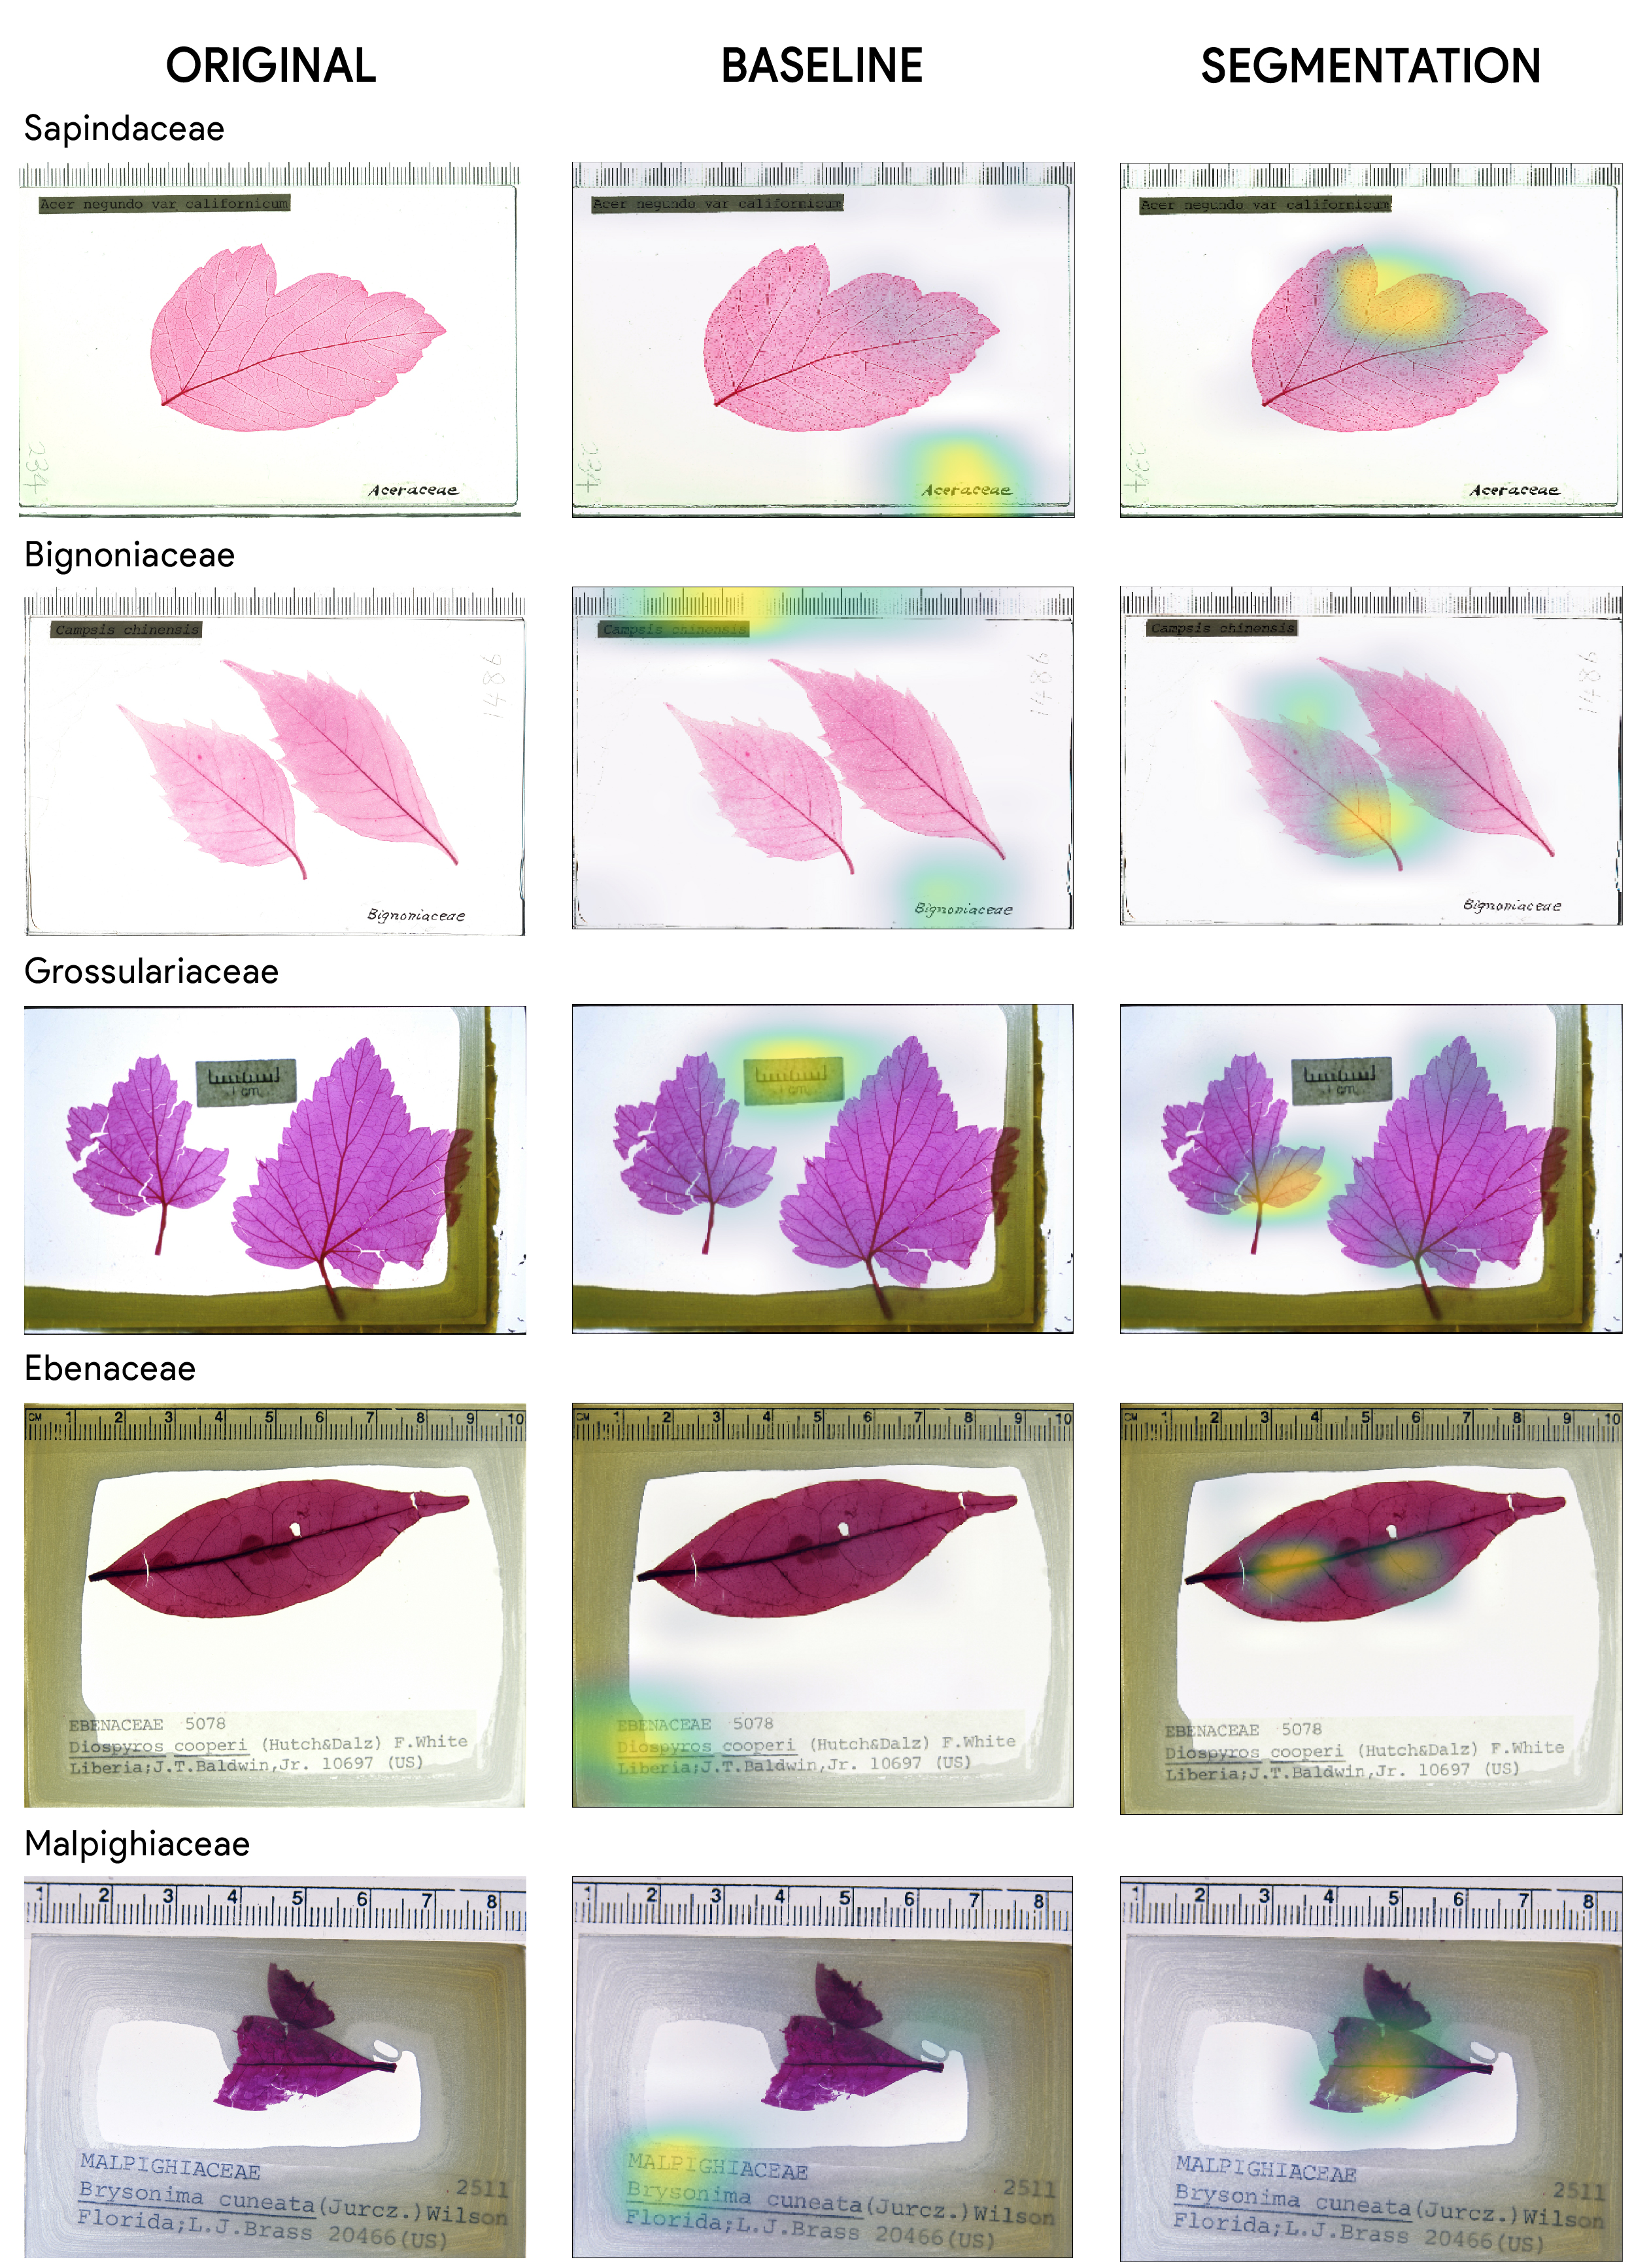
\includegraphics[width=0.88\linewidth]{Figures/SI_Gradcam.jpg}
    \caption{Grad-CAM attribution maps before and after segmentation. 
    \textbf{Left:} Original images. \textbf{Middle:} Attributions without 
    segmentation show reliance on rulers, text, and background artifacts. 
    \textbf{Right:} Attributions with segmentation focus on leaf morphology, 
    eliminating spurious shortcuts.}
    \label{fig:attribution_maps}
\end{figure}


\subsubsection*{Extended Concept Visualization}
Representative examples of additional visual concepts discovered by the 
sparse dictionary learning approach are shown in Figs.~\ref{fig:SI_concepts}--\ref{fig:SI_concepts2}. The complete set of 2048 concepts 
with family-specific importance scores, spatial activation maps, and feature 
visualizations is available at \url{https://serre-lab.github.io/LeafLens/}.


\clearpage


\begin{figure}
    \centering
    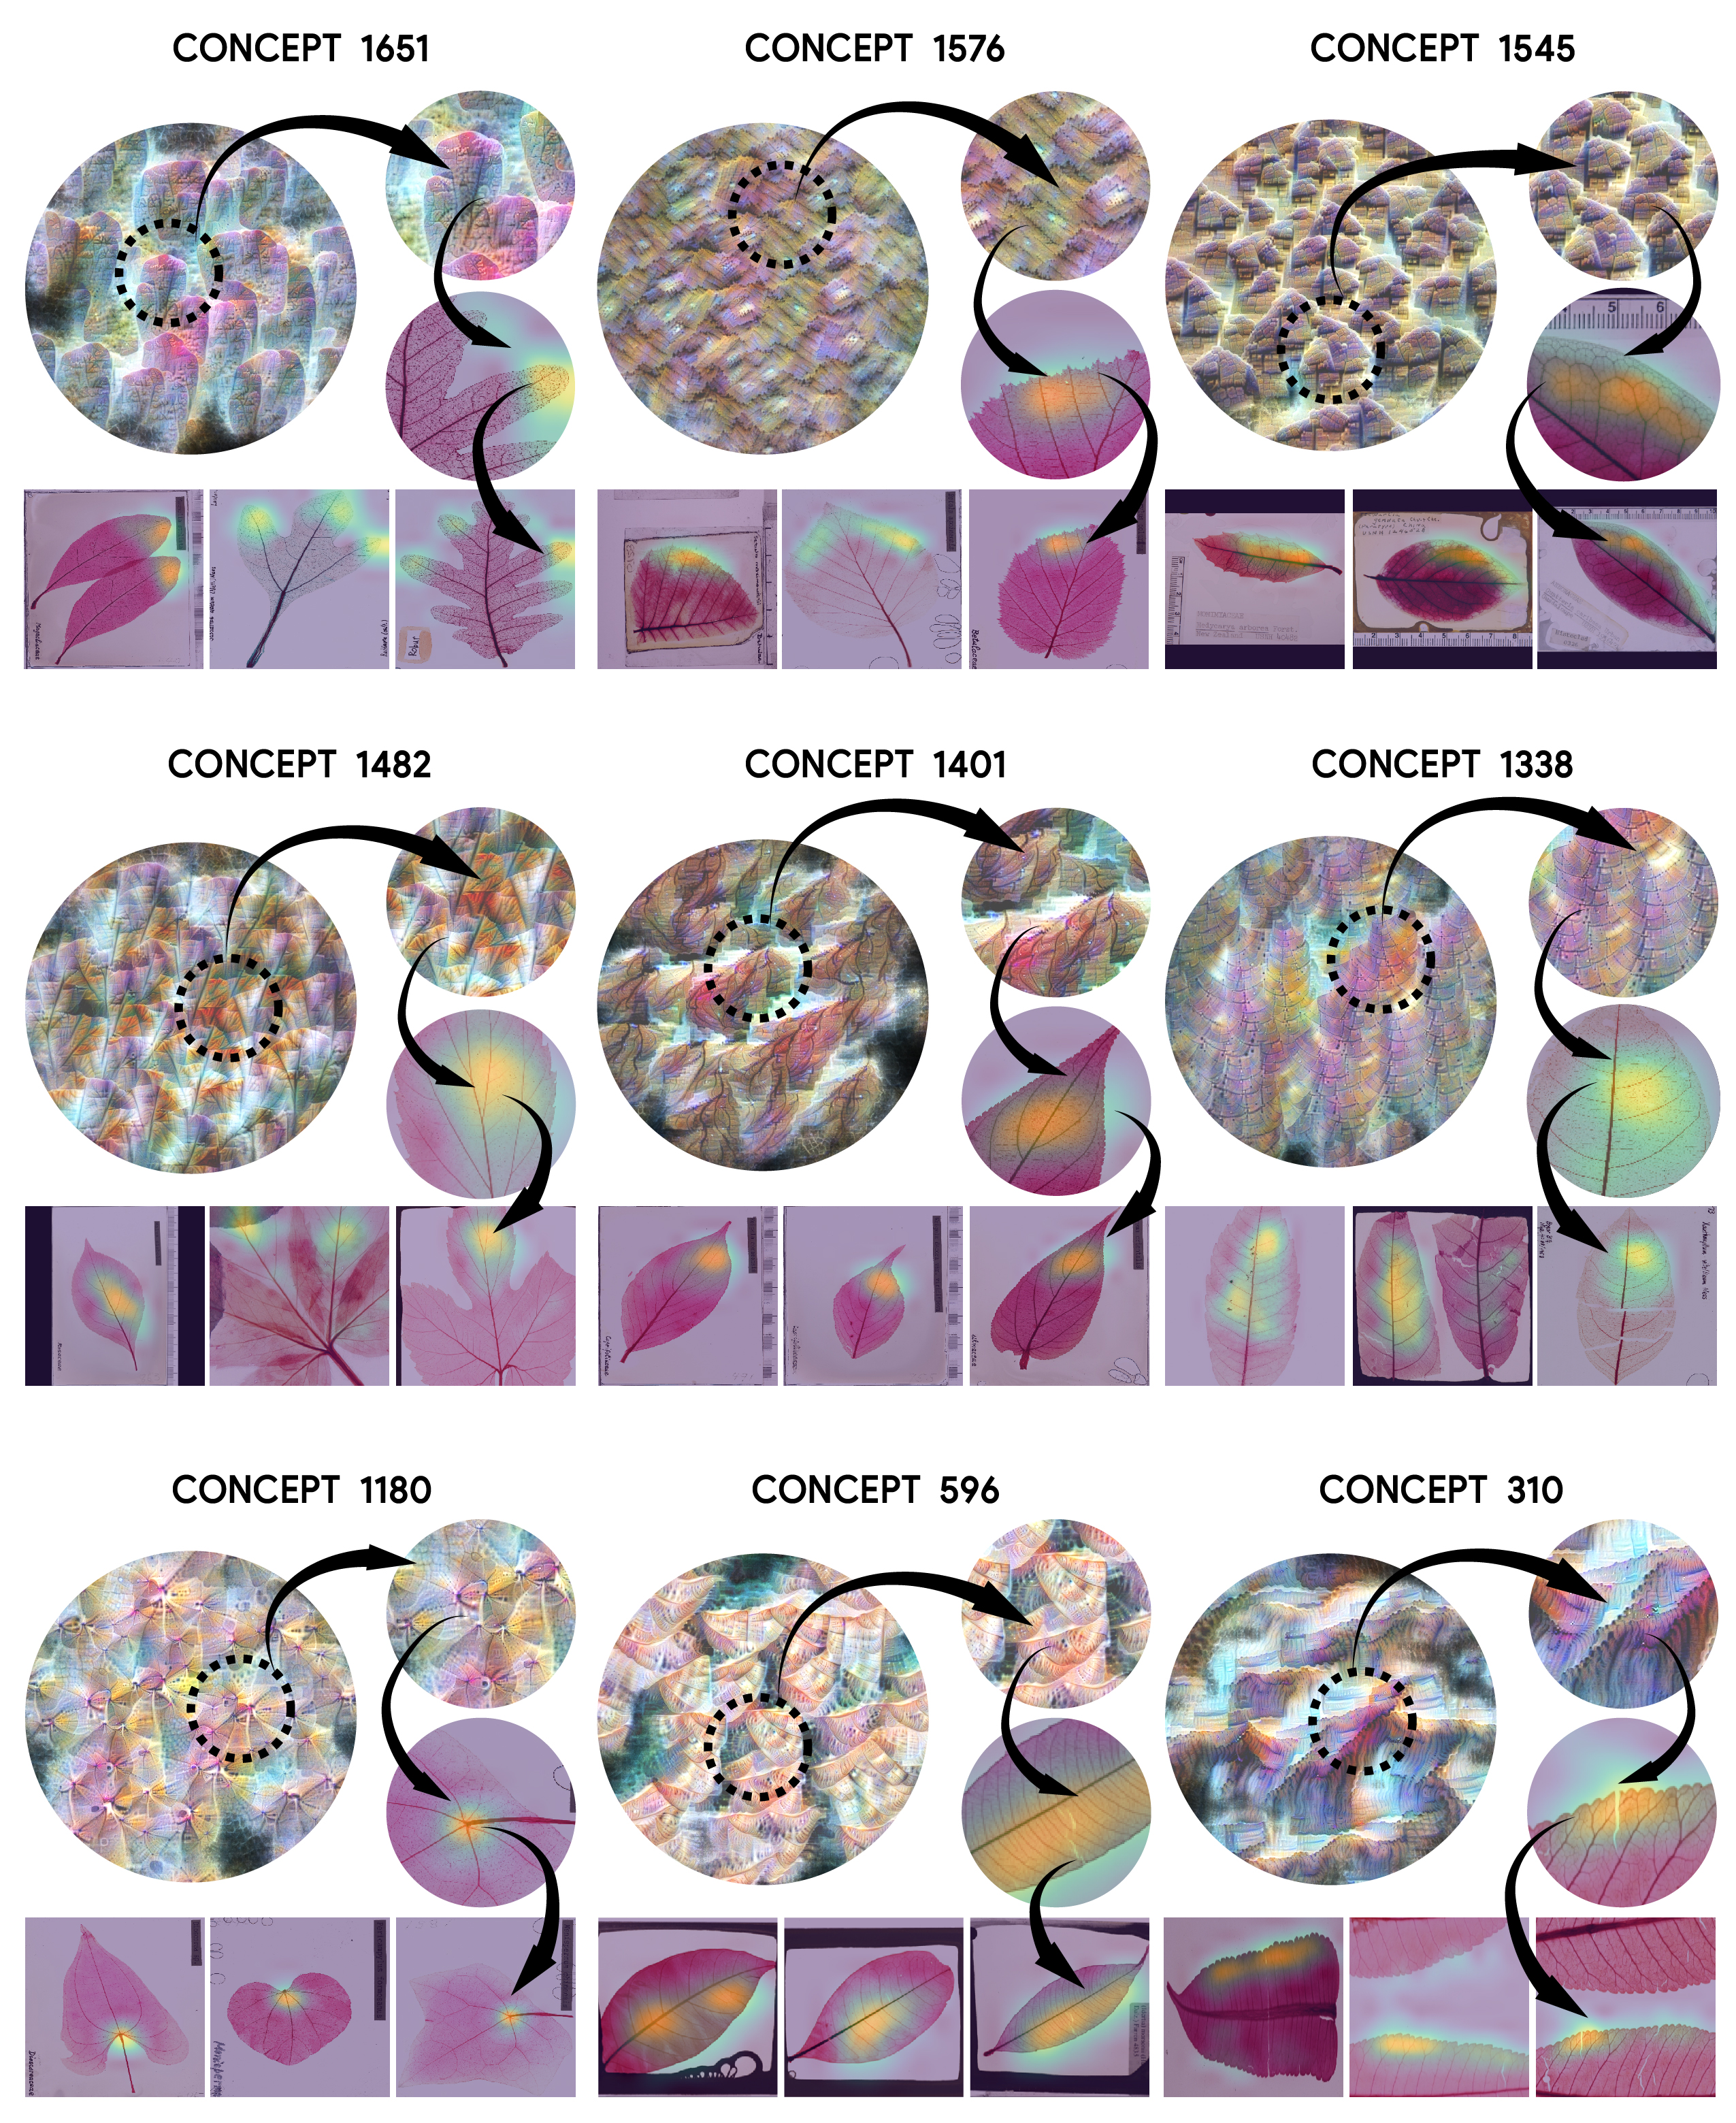
\includegraphics[width=0.88\linewidth]{Figures/SI_6A.jpg}
\caption{Additional examples of visual concepts extracted via sparse dictionary learning. 
Each row shows a different concept with its feature visualization 
revealing the morphological pattern, followed by three attribution maps on representative 
specimens showing where the concept activates. Concepts capture diverse morphological features, 
including venation architecture, leaf margins, tissue texture, and base morphology. See 
Fig.~\ref{fig:SI_concepts2} for more examples. The complete set of extracted concepts with 
family-specific importance scores is available at \url{https://serre-lab.github.io/LeafLens/}.}
\label{fig:SI_concepts}
\end{figure}


\begin{figure}
    \centering
    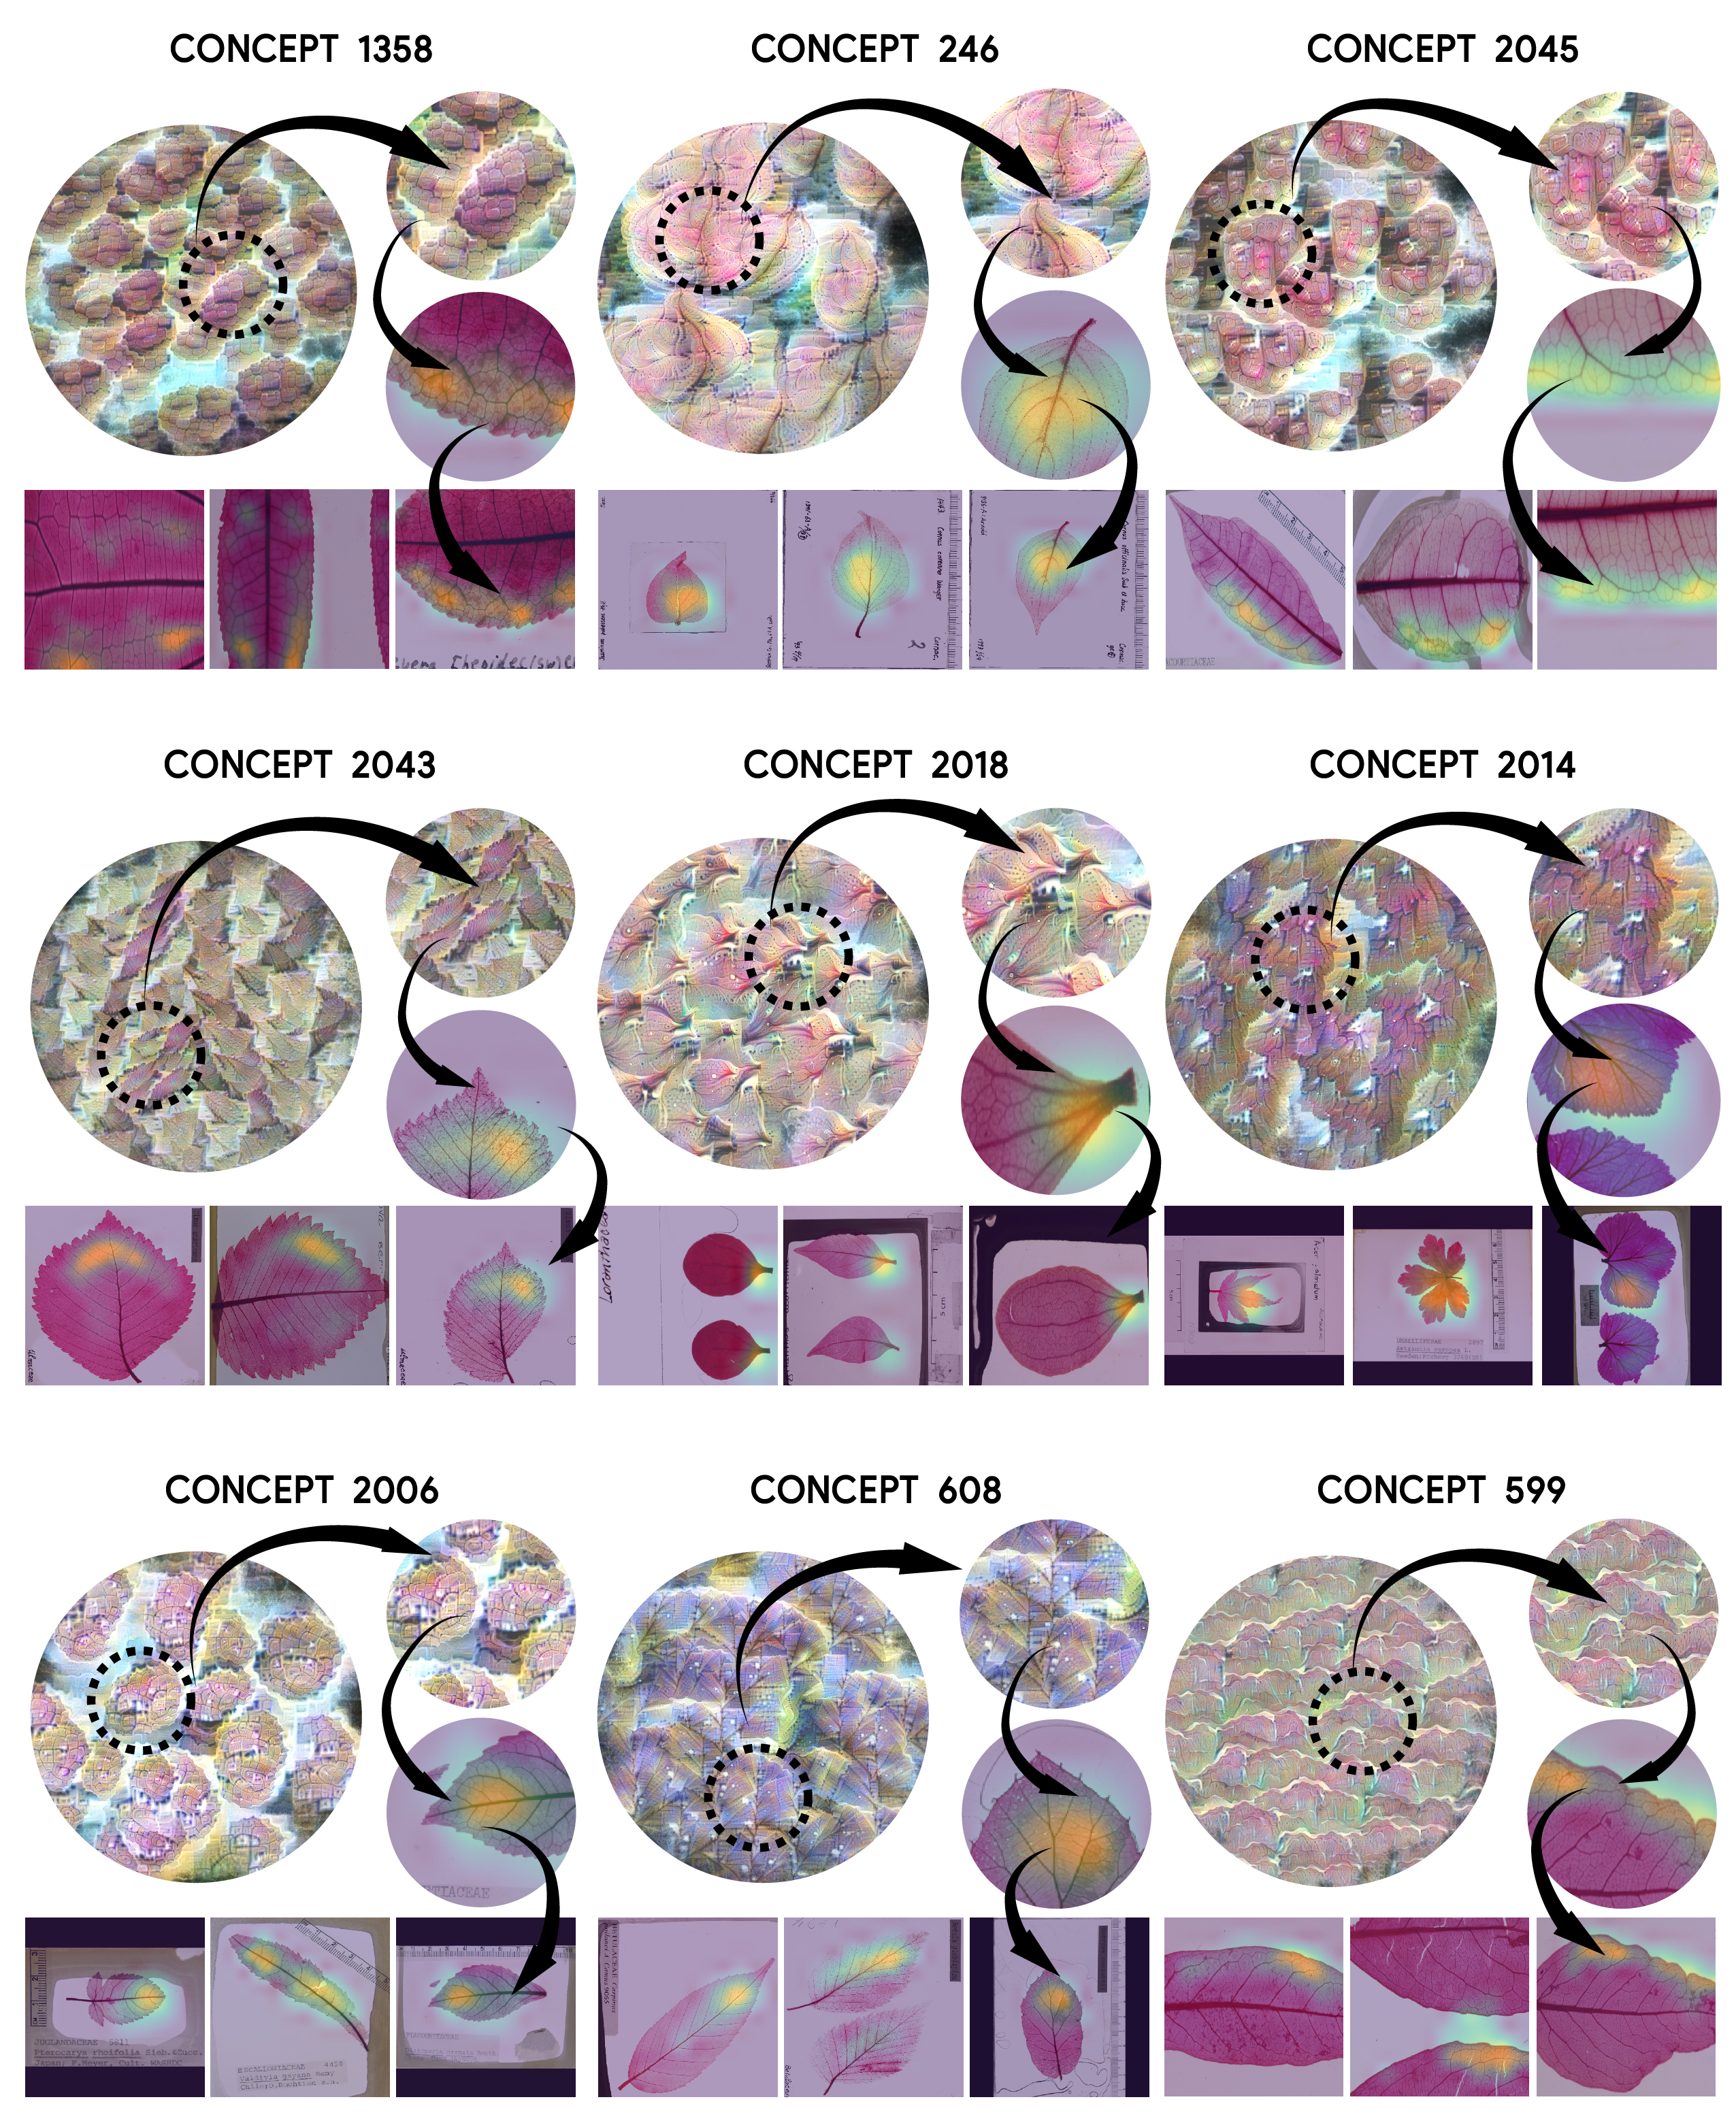
\includegraphics[width=0.88\linewidth]{Figures/SI_6B.jpg}
 \caption{Additional examples of visual concepts extracted via sparse dictionary learning 
(continued from Fig.~\ref{fig:SI_concepts}). Format is identical: feature visualization followed by three attribution maps showing concept activation on actual 
specimens. These examples illustrate the diversity of morphological patterns learned by 
the model, from fine-scale venation details to overall leaf architecture.}
\label{fig:SI_concepts2}
\end{figure}

% \bibliographystyle{sn-mathphys}
% \bibliography{sn-bibliography}% common bib file

%% if required, the content of .bbl file can be included here once bbl is generated
%%\input sn-article.bbl

\end{oldappendices}
\end{document}